\documentclass[a4paper, 12pt]{article}

%----------------------Packages généraux------------------------------

\usepackage[english]{babel}
\usepackage[T1]{fontenc}
\usepackage{ae}
\usepackage[utf8]{inputenc}
\usepackage{vmargin}
\usepackage{hyperref}

%\setmarginsrb{1.75cm}{1cm}{1.75cm}{1cm}{1cm}{0.5cm}{1cm}{0.5cm}
%1 est la marge gauche
%2 est la marge en haut
%3 est la marge droite
%4 est la marge en bas
%5 fixe la hauteur de l'entête
%6 fixe la distance entre l'entête et le texte
%7 fixe la hauteur du pied de page
%8 fixe la distance entre le texte et le pied de page

%----------------------------Mathématiques----------------------------

\usepackage{amsmath}
\usepackage{amssymb}
\usepackage{amsthm}
\usepackage{amsfonts}
\usepackage{eucal}

%----------------------------Bibliographie---------------------------

%\usepackage{cite}
\usepackage[backend=biber,style=ieee,sorting=none,%
    isbn=false,url=false,doi=false,firstinits=true]{biblatex}
\usepackage{filecontents}
\usepackage{hyperref}
\addbibresource{mybib.bib}


%------------------------------Graphics------------------------------

\usepackage{comment}
\usepackage{graphicx}
\usepackage{fancyhdr}
\usepackage{fancybox}
\usepackage{color}
\usepackage{epstopdf}
\usepackage{float}
\usepackage{diagbox}
\usepackage[justification=centering]{caption}
\usepackage{float}
\usepackage{tikz}
\usepackage{subcaption}

%------------------------------Syntaxe------------------------------

\usepackage{listings}
\lstloadlanguages{C}

\setlength{\parindent}{0.5cm}
\setlength{\parskip}{1ex plus 0.5ex minus 0.2ex}
\newcommand{\HRule}{\rule{\linewidth}{0.5mm}}


\definecolor{mygreen}{rgb}{0,0.6,0}
\definecolor{mygray}{rgb}{0.5,0.5,0.5}
\definecolor{mymauve}{rgb}{0.58,0,0.82}
\usepackage{enumitem}
\setlist[itemize]{topsep = 3pt}

\lstdefinestyle{customc}{
  belowcaptionskip=1\baselineskip,
  breaklines=true,
  frame=L,
  xleftmargin=\parindent,
  language=C,
  showstringspaces=false,
  basicstyle=\footnotesize\ttfamily,
  commentstyle=\color{mygreen},
  frame=single,	
  keywordstyle=\bfseries\color{mymauve},
  commentstyle=\itshape\color{mygreen},
  identifierstyle=\color{blue},
  stringstyle=\color{mygray},
}
\lstset{escapechar=@,style=customc}

%Nouvelles commandes
%double souligné
\newcommand{\Bo}{\underline{\underline{B_0}}}
\newcommand{\Ko}{\underline{\underline{K_0}}}
\newcommand{\xo}{\underline{x_0}}
\newcommand{\x}{\underline{x}}

\newcommand{\Bel}{\underline{\underline{B_{el}}}}
\newcommand{\Kel}{\underline{\underline{K_{el}}}}
\newcommand{\B}{\underline{\underline{B}}}
\newcommand{\dK}{\Delta\underline{\underline{K}}}
\newcommand{\II}{\underline{\underline{I}}} %Matrice unitaire I

\newcommand{\I}{\int\limits_0^L}
\newcommand{\SigA}{\sigma_{\alpha}}
\newcommand{\AutoCor}{\sigma_{\alpha}^2 e^{\frac{-|\Delta(s)|}{l}}}
\newcommand{\IntEspCor}{2\sigma_{\alpha}^2\frac{l^2}{L^2}\left(e^{\frac{-L}{l}}+\frac{L}{l}-1\right)}
\newcommand{\EspAlpha}{-\sigma_{\alpha}^2+2\sigma_{\alpha}^2\frac{l^2}{L^2}\left(e^{\frac{-L}{l}}+\frac{L}{l}-1\right)}
\newcommand{\OU}{\text{ }|\text{ }}

\newcommand{\png}[3]{\begin{figure}[H]
    \centering
    \includegraphics[scale = 0.33]{#1.png}
    \caption{#2}
    \label{#3}
\end{figure}}

\newcommand{\myref}[2]{\href{#1}{\textcolor{blue}{\underline{#2}}}}

\newcommand{\tab}[1]{\hspace{.022\textwidth}\rlap{#1}}

\begin{document}

\begin{titlepage}

  	\begin{center} 

    	% top part of the page. The '~' is needed because \\
    	% only works if a paragraph has started.
	
    
\includegraphics[scale=0.35]{logo_fsa.png}  %A changer : image hec
    
\includegraphics[scale=0.6]{logo_Ulg.png}\\[1.15cm]
   		\textsc{\Large First Version}\\[1.2cm]

    	% Title
    	\HRule 
    	\\[0.4cm]
    	{\bfseries \LARGE     Master Thesis
    	\\[0.4cm] 

    	\HRule} \\[2cm]
    	
    % Author and supervisor
    \begin{minipage}{0.4\textwidth}
      \begin{flushleft} \large
         Stassen Théo (s150804)
      \end{flushleft}
    \end{minipage}
    \begin{minipage}{0.4\textwidth}
      \begin{flushright} \large
        \emph{Promoter :} D. Ernst \\      
      \end{flushright}
    \end{minipage}

    \vfill

    % Bottom of the page
    \large 2019-2020

  \end{center}
\end{titlepage}

\newpage


\section{Introduction and problem definition} \label{part1}

\subsection{Introduction} \label{intro}

\textit{Blacklight Analytics} is a enterprise that develop solutions regarding the management of electrical distribution networks. 
Distribution systems
need to integrate more and more renewable generation in their network. Since networks cannot be quickly upgraded and at low cost, new generators are connected to the network under non-firm access contract. The assets used in networks have been designed to transmit power in one direction, from the global network to the local network. This configuration implies situations where the high production creates congestion problems in the assets, while energy generated must be injected into the global network . There is
a need for a practical method able to compute the production limits of the generators such that the system can be considered safe, i.e has a very low probability that the electrical power flowing through one asset is higher than the maximum tolerated power is this asset.


Blacklight Analytics develops a solution to 
this problem. The method cast the problem into a stochastic decision process. This process is divided in three phases : (i) generation of a network model, (ii) forecasting of the power produced or consumed and (iii) computation of the generator limits. The phase 2 takes as input historical measurements of the networks and output future production probability distribution for each sources. This output will be used to define generator limits.
In the current implementation, the forecasting method uses Gaussian process regression to forecast individually each source and combine information using covariance estimation. 
This master thesis subject addresses the question of what is the best forecasting method to implement in this described context, and what are the elements of comparison that allows us to make these affirmation. The growing scientific field of Deep Learning has a great potential to be exploited to achieve this goal. 

Therefore, the concrete goal of this Master Thesis is the comparison of different probabilistic forecasting models and techniques, mostly from the deep learning scientific field,
in the context of the prediction of renewable energy production.

\subsection{Related Works}


Time series forecasting is a well-defined and extensively explored scientific field. It is considered as part of the probabilities scientific field for many years, from very simple or naive forecasting models (\textit{Naive}, \textit{Seasonal Naive}, \textit{Moving Average}, etc) \cite{forecasting_principle1} to more complex models as the \textit{Autoregressive integrated moving average} (\textit{ARIMA}) \cite{forecasting_principle2} or \textit{Exponential smoothing}, introduced by statistician Robert Goodell Brown in 1956 \cite{smooth_for}.
\textit{Exponential smoothing} and \textit{ARIMA} models are the two most widely used approaches to time series forecasting, and provide complementary approaches to the problem. While \textit{exponential smoothing} models are based on a description of the trend and seasonality in the data, \textit{ARIMA} models aim to describe the autocorrelations in the data.

Probabilistic time series forecasting stems from point time series forecasting. For instance, \textit{ETS} forecasting is an \textit{exponential smoothing} method that can generate point but also intervals prediction \cite{exp_smooth}. 

In recent years, advances in deep learning has led to interesting results in probabilistic forecasting field. Recent publications (\cite{deep_factors_gp}, \cite{multi_horizon_quantile}) and forecasting competitions results (\cite{extreme_event_for_nn}, \cite{m4_competition})  have shown the relevance of using deep learning based models to obtain better results than with ETS or ARIMA methods.

Deep Learning probabilistic forecasting of renewable energy production is a subject that has already been covered by various scientific teams, with different contexts, goals and techniques. These various results has been compiled and analysed in different scientific review papers. Probabilistic forecasting in the context of wind turbines generation has been reviewed in \cite{review_prob_for_wind}. Deep learning techniques for renewable energy forecasting has been reviewed in \cite{review_deep_renewable_for}. These reviews exposes notably a great number of different models.

Regarding the implementation of these techniques, deep learning frameworks, such as \textit{Tensorflow} \cite{tensorflow}, \textit{MXNet} \cite{mxnet} and \textit{Pytorch} \cite{pytorch} are popular solutions. Considering  the time series modeling, a  number of  commercial and open-source solutions exist but does not provides toolkits focused on modern deep learning.  For example the  \textit{R-forecast}  package  \cite{r_article}  provide a plethora of models and tooling for classical forecasting methods and contains neural forecasting models, however these pre-date modern deep learning methods and only contain stand-alone implementations of simple local models, they lack state-of-the-art architectures. 
This lack of specific toolkit has been recently filled with \textit{GluonTS} (\url{https://gluon-ts.mxnet.io}) \cite{gluontsbible}, a deep learning library that bundles components, models and tools for time series applications such as point and probabilistic forecasting or anomaly detection. It relies on the deep-learning framework MXNet, developed by \textit{Amazon Web Services}.
As it provides all the services needed to produce experiments and comparison of deep learning probabilistic forecasting models, it is the main implementation tool of this master thesis.


\subsection{Problem Statement} \label{problem_statement}

Before entering into solution description, we need to define mathematically in general the problem of time series deep-learning forecasting, whereabouts \textit{GluonTS} has been conceived. 

As different types of models has fundamental differences in the way they express the problem, the mathematical formulation differs.
Two mathematical formulation are presented, corresponding to two types of models found among the implemented models.
The first mathematical formulation corresponds to the feed-forward models.
The second mathematical formulation corresponds to the RNN models. 

Models data is composed of certain number of time series in training data and in testing data. 
In general the training and testing data is composed of the same time series (this affirmation is discussed in section \ref{datasets}). This situation is the one considered in this section.

Let the following variables :

\begin{itemize}%[label=$*$]
    \item $I$ the number of time series considered
    \item $T$ the number of time steps in time series
    %\item T the number of time steps in time series
    \item $x_{i,t}$ a scalar variable representing the value of the time series i at time step t.
    %\item $\hat{x}_{i,t}$ a scalar variable representing the predicted value of the time series i at time step t.
    %\item $\phi(x_{i,t}) : \mathbb{R} \to \mathbb{R}$, the density probability function of the variable $x_{i,t}$, which associate to a value of $x_{i,t}$ the corresponding probability.
    %\item $\hat{\phi}(x_{i,t}) : \mathbb{R} \to \mathbb{R}$, the predicted density probability function of the variable $x_{i,t}$, which associate to a value of $x_{i,t}$ the corresponding probability.
    \item $a, b, c, d, e$ specific values of $t$, with $e=T$
    \item $t=0 < t=a < t=b < t=c < t=d < t=e$
    \item $predict\_length = b-a$, fixed hyper parameter of the problem.
    Indicates the number of time steps about which the models must make a prediction simultaneously.
    \item $context\_length = c-b$, fixed hyper parameter of the problem.
    Indicates the number of time steps that the model consider as input simultaneously.
    %\item $\text{NN}_\theta : \mathbb{R}^n \to \mathbb{R}^m$,  the neural network, viewed as a function taking a vector of n values
    %as input and giving a vector of m values of density of probability as output.
    %\item $L : \mathbb{R} \times (\mathbb{R} \to \mathbb{R} ) \to \mathbb{R} $ the loss function taking a value and a density of probability as input and giving a loss value as output.
    %The details of loss implementation are discussed in section \ref{loss}, the loss choose coming from the discussion about project goal in section \ref{goal}.
    %\item $M([\phi_{x_P1},..,\phi_{x_Pn}],[{x_{O1}},..,{x_{On}}])$  the metric function which
    %gives the value of metric for a vector of density of probability of predicted value of the variable x and  the corresponding vector of observed values of the variable x. 
    %The details of metrics function are discussed in section \ref{metrics}

\end{itemize}

We also define $L : \mathbb{R} \times (\mathbb{R} \to \mathbb{R} ) \to \mathbb{R} $ the loss function taking a value and a probability distribution as input and giving a loss value as output,
As example of function L, we can mention the negative log-likelihood :

\begin{equation}
    L(y, \phi(x) ) = - ln(\phi(x = y) )
\end{equation}

The details of loss implementation are discussed in section \ref{loss}.


Each time series can be conceptually decomposed as two pieces. The first piece, $[x_{i,0},...,x_{i,d-1}]$  correspond to the part of the time series whereupon we want to train. The second piece $[x_{i,d},...,x_{i,e-1}]$ correspond to the part of the time series whereupon we want to test.
The training set is composed only of the first pieces of each time series when the training set is composed of the two pieces (i.e. the totality of the time series).

At the end of the training, the model neural network has been trained on the whole training data, and can be tested on the testing data. 

%Depending of the type of model used, there are some significant differences in expressions. 
%Two main cases are presented, the feed-forward models case (which belongs to the generative models category) and the RNN models case (which belongs to the discriminative models category).


 %In contrast to classical model approach like ETS and ARIMA, which consider functions per time series individually, neural models further express one function, as a neural network, whose weights are trained among all time series given as input. The model learn from the whole training data. Each time series can be tested using this trained neural network.


\subsubsection{First mathematical formulation : Feed Forward models}

This formulation corresponds to the way the models that can be described as Feed Forward (\textit{Simple} and \textit{SimpleFeedForward }) compute a solution of the problem.

\begin{figure}[H]
\centering
\begin{center}
\begin{tikzpicture}
\draw (-1,0) -- (-1,3);
\draw (10,0) -- (10,3);
\draw (-1,0) -- (10,0);
\draw (-1,3) -- (10,3);
\draw [very thin, blue] (3,0) -- (3,3);
\draw [very thin, cyan] (6,0) -- (6,3);
\draw [very thin, blue] (7,0) -- (7,3);
\draw [red] (9,0) -- (9,3);
\draw (-1,1.5) node [left] {$x_i$};
\draw (-1,3) node [above] {$0$};
\draw (3,3) node [above] {$a$};
\draw (6,3) node [above] {$b$};
\draw (7,3) node [above] {$c$};
\draw (9,3) node [above] {$d$};
\draw (10,3) node [above] {$e$};
\draw [<->, blue] (2.5,1.5) -- (3,1.5);
\draw [<->, blue] (7,1.5) -- (7.5,1.5);
\draw [help lines, dashed,ystep=10,xstep=0.5] (-1,0) grid(10,3);
\end{tikzpicture}
\end{center}
\caption{Feed forward models forecast : General case}
\label{fig:forecast1_gen}
\end{figure}


Considering an interval $[x_{i,a},...,x_{i,c-1}]$ in the time series i,
our goal is to estimate the distribution of future window $[x_{i,b},...,x_{i,c-1}]$ given its history $[x_{i,a},...,x_{i,b-1}]$. The estimated distribution is defined as :

\begin{equation} \label{distrib_proba_equ}
    p_{\theta}(x_{i,b}, ..., x_{i,c-1} | x_{i,a}, ..., x_{i,b-1}) 
\end{equation}

Where $\theta$ denotes the models parameters.
This distribution can be factorised as :

\begin{equation} \label{distrib_proba_fact_equ}
    p_{\theta}(x_{i,b}, ..., x_{i,c-1} | x_{i,a}, ..., x_{i,b-1}) =
    \prod_{t=b}^{c-1}p_{\theta}(x_{i,t} | x_{i,a}, ..., x_{i,b-1})
\end{equation}


We define $\text{NN}_\theta$, a neural network parametrized by $\theta$. It hypothesis space is defined as $\{ h : \mathbb{R}^{b-a} \to R ^{k(c-b)}, h \in H \}$. With k the number of parameters needed to defines the output distribution. 
We consider the case of a gaussian distribution, with $k=2$. The evaluation of $\text{NN}_\theta$ can be described as :


\begin{equation}
    [\mu_{\theta i,b},..,\mu_{\theta i,c-1},\sigma_{\theta i,b},..,\sigma_{\theta i,c-1}] = \text{NN}_\theta({x_{i,a}},..,{x_{i,b-1}})
\end{equation}


%The goal is the approximation of hidden variables $[{\phi}(x_{i,b-a}),..,{\phi}(x_{i,d-1})]$ :

%\begin{equation}
%    [\hat{\phi}(x_{i,b-a}),.., \hat{\phi}(x_{i,d-1})]  \approx [{\phi}(x_{i,b-a}),..,{\phi}(x_{i,d-1})] \forall i \in [1,I]
%\end{equation}


%The training of the neural network is composed of a succession of training steps involving one neural network prediction. The hypothesis space \textit{H} explored by this neural network N  is defined as \{$ h : \mathbb{R}^{b-a} \to (\mathbb{R} \to \mathbb{R} )^{c-b}, h \in H $\}.

%A training step is mathematically defined in the following equation :

%\begin{equation}
%    [\hat{\phi}(x_{i,b}),..,\hat{\phi}(x_{i,c-1})] = N({x_{i,a}},..,{x_{i,b-1}}), a \in [0, d - (c-a)],  i \in [1,I]
%\end{equation}

%The hypothesis space \textit{H} explored by the neural network $\text{NN}_\theta$ parametrized by $\theta$  is defined as \{$ h : \mathbb{R}^{b-a} \to R ^{2(c-b)}, h \in H $\}.

The estimated distribution of a variable $x_{i,t}$ of the future window ($t \in [b,c-1]$) is expressed as, with $\phi_{\mu,\sigma}: \mathbb{R} \to \mathbb{R} $ a gaussian function parametrized by parameters $\mu$ and $\sigma$ :

\begin{equation}
    p_{\theta}(x_{i,t} | x_{i,a}, ..., x_{i,b-1}) = \phi_{\mu_{\theta i,t},\sigma_{\theta i,t}}(x_{i,t})
\end{equation}

The estimated distribution of the future window as defined in equation \ref{distrib_proba_equ} is expressed as :

\begin{equation}
    p_{\theta}(x_{i,b}, ..., x_{i,c-1} | x_{i,a}, ..., x_{i,b-1})  = \prod_{t=b}^{c-1}\phi_{\mu_{\theta i,t},\sigma_{\theta i,t}}(x_{i,t})
\end{equation}



This estimation is performed for different intervals $[x_{i,a},...,x_{i,c-1}]$. We consider disjoint adjacent future windows, from the first possible future window $(b = context\_length)$, see figure \ref{fig:forecast1_start}, to the last possible future window $(b=d-predict\_length)$, see figure \ref{fig:forecast1_last}, and for all time series $i \in [0,I]$.
 
 \begin{figure}[H]
\centering
\begin{center}
\begin{tikzpicture}
\draw (-1,0) -- (-1,3);
\draw (10,0) -- (10,3);
\draw (-1,0) -- (10,0);
\draw (-1,3) -- (10,3);
\draw [very thin, blue] (-1,0) -- (-1,3);
\draw [very thin, cyan] (2,0) -- (2,3);
\draw [very thin, blue] (3,0) -- (3,3);
\draw [red] (9,0) -- (9,3);
\draw (-1,1.5) node [left] {$x_i$};
\draw (-1,3) node [above] {$a = 0$};
\draw (2,3) node [above] {$b$};
\draw (3,3) node [above] {$c$};
\draw (9,3) node [above] {$d$};
\draw (10,3) node [above] {$e$};
\draw [help lines, dashed,ystep=10,xstep=0.5] (-1,0) grid(10,3);
\end{tikzpicture}
\end{center}
\caption{Feed forward models forecast : First possible interval}
\label{fig:forecast1_start}
\end{figure}

\begin{figure}[H]
\centering
\begin{center}
\begin{tikzpicture}
\draw (-1,0) -- (-1,3);
\draw (10,0) -- (10,3);
\draw (-1,0) -- (10,0);
\draw (-1,3) -- (10,3);
\draw [very thin, blue] (0,0) -- (0,3);
\draw [very thin, cyan] (3,0) -- (3,3);
\draw [very thin, blue] (4,0) -- (4,3);
\draw [red] (9,0) -- (9,3);
\draw (-1,1.5) node [left] {$x_i$};
\draw (-1,3) node [above] {$0$};
\draw (0,3) node [above] {$a$};
\draw (3,3) node [above] {$b$};
\draw (4,3) node [above] {$c$};
\draw (9,3) node [above] {$d$};
\draw (10,3) node [above] {$e$};
\draw [help lines, dashed,ystep=10,xstep=0.5] (-1,0) grid(10,3);
\end{tikzpicture}
\end{center}
\caption{Feed forward models forecast : Second possible interval}
\label{fig:forecast1_second}
\end{figure}

\begin{figure}[H]
\centering
\begin{center}
\begin{tikzpicture}
\draw (-1,0) -- (-1,3);
\draw (10,0) -- (10,3);
\draw (-1,0) -- (10,0);
\draw (-1,3) -- (10,3);
\draw [very thin, blue] (5,0) -- (5,3);
\draw [very thin, cyan] (8,0) -- (8,3);
\draw [very thin, blue] (8.99,0) -- (8.99,3);
\draw [red] (9,0) -- (9,3);
\draw (-1,1.5) node [left] {$x_i$};
\draw (-1,3) node [above] {$0$};
\draw (5,3) node [above] {$a$};
\draw (8,3) node [above] {$b$};
\draw (9,3) node [above] {$c = d$};
\draw (10,3) node [above] {$e$};
\draw [help lines, dashed,ystep=10,xstep=0.5] (-1,0) grid(10,3);
\end{tikzpicture}
\end{center}
\caption{Feed forward models forecast : Last possible interval}
\label{fig:forecast1_last}
\end{figure}


Finally, the global loss of the estimation is defined as the sum, for each time series and each time step,  of the loss function $L$ with as argument the real value and the estimated distribution :


\begin{equation}
    loss(\theta) = \sum^{I}_{i=1}\sum^{d-1}_{t=b-a}L(x_{i,t},\phi_{\mu_{\theta i,t},\sigma_{\theta i,t}}(x_{i,t}))
\end{equation}



%These training steps are performed for each possible value of \textit{a}, and for each possible value of \textit{i}.



%The final loss evaluated during training is defined as, with $\theta$ the parameters of the neural network N :

%\begin{equation}
%    loss(\theta) = \sum^{I}_{i=1}\sum^{d-1}_{t=b-a}L(x_{i,t},\hat{\phi}(x_{i,t}))
%\end{equation}



\subsubsection{Second mathematical formulation : RNN models}

This formulation corresponds to the way the models that can be described as RNN (\textit{CanonicalRNN}) express the problem.

\begin{figure}[H]
\begin{center}
\begin{tikzpicture}
\draw (-1,0) -- (-1,3);
\draw (10,0) -- (10,3);
\draw (-1,0) -- (10,0);
\draw (-1,3) -- (10,3);
\draw [very thin, blue] (3,0) -- (3,3);
\draw [very thin, blue] (7,0) -- (7,3);
\draw [red] (9,0) -- (9,3);
\draw (-1,1.5) node [left] {$x_i$};
\draw (-1,3) node [above] {$0$};
\draw (3,3) node [above] {$a$};
\draw (7,3) node [above] {$c$};
\draw (9,3) node [above] {$d$};
\draw (10,3) node [above] {$e$};
\draw [<->, blue] (2.5,1.5) -- (3,1.5);
\draw [<->, blue] (7,1.5) -- (7.5,1.5);
\draw [help lines, dashed,ystep=10,xstep=0.5] (-1,0) grid(10,3);
\end{tikzpicture}
\end{center}
\caption{RNN models forecast: General case}
\label{fig:forecast2_gen}
\end{figure}

%The goal is the approximation of hidden variables $[{\phi}(x_{i,0}),..,{\phi}(x_{i,d-1})]$ :

Considering an interval $[x_{i,a},...,x_{i,c-1}]$ in the time series i,
our goal is to estimate the distribution of window $[x_{i,a},...,x_{i,c-1}]$ given its hidden states $[h_{i,a},...,h_{i,c-1}]$. The estimated distribution is defined as :

\begin{equation} \label{distrib2_proba_equ}
    p_{\theta}(x_{i,a}, ..., x_{i,c-1} | h_{i,a}, ..., h_{i,c-1}) 
\end{equation}

Where $\theta$ denotes the models parameters.
This distribution can be factorised as :

\begin{equation} \label{distrib2_proba_fact_equ}
    p_{\theta}(x_{i,a}, ..., x_{i,c-1} | h_{i,a}, ..., h_{i,c-1})  =
    \prod_{t=a}^{c-1}p_{\theta}(x_{i,t} | h_{i,a}, ..., h_{i,t})
\end{equation}

We define $f_\theta$, a function parametrized by $\theta$. It hypothesis space is defined as $\{ h_f : \mathbb{R} \cross \mathbb{R} \to \mathbb{R} , h_f \in H_f \}$.
It evaluation can be described as, for $t \in [a+1,c-1]$  :

\begin{equation}
    h_{i,t} = f_\theta({x_{i,t}},h_{i,t-1})
\end{equation}

We define $\text{g}_\theta$, a function parametrized by $\theta$. It hypothesis space is defined as $\{ h_g : \mathbb{R} \to \mathbb{R}^k , h_g \in H_g \}$. With k the number of parameters needed to defines the output distribution. 
We consider the case of a gaussian distribution, with $k=2$.
It evaluation can be described as, for $t \in [a+1,c-1]$ ::

\begin{equation}
    [\mu_{\theta i,t}, \sigma_{\theta i,t}] = g_\theta(h_{i,t})
\end{equation}

The estimated distribution of a variable $x_{i,t}$ of the interval ($t \in [a,c-1]$) is expressed as, with $\phi_{\mu,\sigma}: \mathbb{R} \to \mathbb{R} $ a gaussian function parametrized by parameters $\mu$ and $\sigma$ :

\begin{equation}
    p_{\theta}(x_{i,t} | h_{i,a}, ..., h_{i,t}) = \prod_{t=b}^{c-1} \phi_{\mu_{\theta i,t},\sigma_{\theta i,t}}(x_{i,t})
\end{equation}

The distribution of interval as defined in equation \ref{distrib2_proba_equ} is expressed as  :

\begin{equation}
     p_{\theta}(x_{i,a}, ..., x_{i,c-1} | h_{i,a}, ..., h_{i,c-1})  = \prod_{t=b}^{c-1} \phi_{\mu_{\theta i,t},\sigma_{\theta i,t}}(x_{i,t})
\end{equation}

This estimation is performed for different intervals $[x_{i,a},...,x_{i,c-1}]$. We consider disjoint adjacent interval, from the first possible future interval $(c = context\_length + predict\_length)$, to last possible future window $(c=d)$, and for all time series $i \in [0,I]$.


Finally, the global loss of the estimation is defined as the sum, for each time series and each time step considered, of the loss function $L$ with as argument the real value and the estimated distribution :

\begin{equation}
    loss(\theta) = \sum^{I}_{i=1}\sum^{d-1}_{t=b-a}L(x_{i,t},\phi_{\mu_{\theta i,t},\sigma_{\theta i,t}}(x_{i,t}))
\end{equation}


%The final loss evaluated during training is defined as, with $\theta$ the parameters of the neural network N :

%\begin{equation}
%    loss = \sum^{I}_{i=1}\sum^{d-1}_{t=0}L(x_{i,t},\hat{\phi}(x_{i,t}))
%\end{equation}



%The neural network is trained by minimization of the loss as mathematically defined here :
%The training pass of the neural network can be seen as the following mathematical expression :



%The goal of the forecasting process is the minimization of this loss.


\section{Second Part : GluonTS}

\subsection{GluonTS historical}

At the time of writing this master thesis, GluonTS is a very recent toolkit, which is coherent with the fact that the deep learning forecasting field is early itself.
It first release version (\textit{v0.1.0}) is dated from March 3rd 2019.
The implementation of the code has been performed on the version \textit{v0.4.2} released on
November 26th 2019 and as been updated for version \textit{v0.5.0}, released on May 12nd 2020.
These versions are/was still considered as beta versions. This implied several bugs and implementation issues. In particular some models (for example an implementation of the \textit{DeepState} model \cite{deepstate_paper})  failed to run correctly, and the run of "custom" models (implemented using the provided model template) is incompatible with the hybridization functionality, which provides important time optimization, because of a bug. 
And some functionalities that would be useful are not currently implemented, as alternative loss functions (see \ref{custom_loss} section).

\subsection{GluonTS Functioning}

The GluonTS toolkit defines a dataset structure, containing in particular the time series. This dataset, is given to a GluonTS model (pre-implemented or implemented using the provided model template), which use the dataset information (to train and test the model). When the model is evaluated, it gives in all cases as output a distribution for each of the testing time steps, for each time series (see \ref{problem_statement}).
The type of output distribution is defined by the user and discussed in section \ref{distribution}. Concretely, the output information is a set of randomly drawn sample of the predicted distribution,
not the distributions parameters themselves.
The model, if belongs to deep learning models category, must be trained before evaluation, using the chosen loss function (see section \ref{loss}).
The resulting output distributions can be evaluated using the appropriate metrics (see section \ref{metrics}).

\subsection{Datasets} \label{datasets}

GluonTS interface imposes a certain structure of datasets, object used for training and testing  models. There are composed of some mandatory and some optional components.
$`dataset.train`$ is an iterable collection of data entries used for training. Each entry corresponds to one time series.  $'dataset.test$ is an iterable collection of data entries used for inference. $`dataset.metadata`$ contains metadata of the dataset such as the frequency of the time series, the context length,  the prediction length.
%associated features. These associated features are data given in addition to the time series, that will also been seen as input by the network. They can be static, dynamic, real, categorical , etc.

%We should emphasize here that a single moded is trained over all the time series contained in the training dataset . This results in a global model, suitable for prediction for all the time series in the testing dataset as it is defined in the classical way and possibly for other unseen related time series.

GluonTS is optimized to handle multiple time series in parallel. The training time will be significantly increased if the dataset is composed of only one time series of very long length compared to a dataset composed of multiples time series of smaller length. 

As mentioned in section \ref{problem_statement}, in general the training and testing set is composed of the same time series.
The definition of the task whereabouts this master thesis is dedicated, the forecasting of wind turbines production, is not compatible with this general affirmation.
In fact, the goal is to forecast the production of an energy generator using a model which couldn't be trained on the current generator production history, but on others generator production history.
It is nowadays useful to test different configurations of training/testing data, including where the training data and testing data comes from the same generator(s) history. This allow us to test how the forecast quality is influenced by the variation of configuration of input data.

Input data provided by "Blacklight Analytics" is composed of different (raw) time series :

\begin{itemize}
    \item A continuous 6 months history of a wind turbine production , in kWh \newline
    (\textit{6months-minutes.csv})
    \item An history of a wind turbine production, in negative MWh \newline 
    (\textit{mesure\_p\_gestamp.csv})
    \item A 2 days history of two wind turbines production, in negative MWh \newline
    (\textit{2eol\_measurements.csv})
\end{itemize}

All the data is at a frequency of 1 minute, and is converted in positive MWh. 
Nowadays the configuration, because of the GluonTS behaviour optimized to handle multiple time series, these original times series are manually splitted before putting them in dataset structure.
Each time series is manually splitted in certain number of time series of same size. This size is considered as a hyper parameter of the problem ($data\_size$). 

The configurations considered are the following :

\begin{itemize}
    \item All the disposable times series are used as training and testing data. It is referred as "Config A"
    \item \textit{2eol\_measurements.csv} time series used as testing data and the other time series as training data. It is referred as "Config B".
\end{itemize}

GluonTS allow the use of "features", i.e. information used as input to the models additionally to time series information. Not all the models are compatible with this functionality. 
In our case, the different sources of information could be identified using static categorical features. For example, in the configuration A, splitted time series coming from time series \textit{6months-minutes.csv} will have a categorical value of 0, time series from \textit{mesure\_p\_gestamp.csv} the value of 1, times series from \textit{2eol\_measurements.csv} values of 2 and 3. This functionality useful if the different sources have significant differences.

The size of the prediction window  \textit{BlackLight Analytics} is interested in is 10 minutes, i.e a predict length of 10  for a frequency of 1 minute. The context length, as defined in section \ref{problem_statement} is a hyper parameter of the problem indicating the number of time steps considered as input for the model network.



\subsection{Quantiles} \label{goal}

GluonTS allow selecting the values of quantiles that will be computed, to evaluate the metrics and to possibly use these information in loss function.
This functionality is used in section \ref{custom_loss}.
%In the current implementation, the value of $e$ is $1\%$, the security quantile is $quantile(0.99)$.

%In current implementation, the value of $e$ is $1\%$ but the security quantile is $quantile(0.995)$ because of a little modification comparing to the goal specified before. The goal currently considered is not only the difference minimization of the "upper" quantile but also the reverse "lower" quantile, concretely $quantile(0.995)$ and $ quantile(0.005)$, in order to obtain a 99\% window as correct as possible. It impacts the formulation of the custom loss and custom metric in respective sections. This must probably be modified to focus only on the $quantile(0.99)$.%
  
  \subsection{Loss} \label{loss}

GluonTS implements in it predefined models only one type of loss function.
This loss function is, for the majority of the models, the inverse of the log-density of the output distribution, as defined in the equation \ref{base_loss_def}. In some models, the fundamental difference in terms of architecture justify a different loss. For example the \textit{MQRNN} and \textit{MQCNN} models use different quantile losses as loss function.


If $\phi(x)$ is the output density distribution and y the observed value, the loss value is : 

\begin{equation} \label{base_loss_def} 
    base\_loss(y, \phi(x) ) = - ln(\phi(x = y) )
\end{equation}


This loss express efficiently that the predicted distribution must corresponds to the real distribution. In the chapter \ref{part3} of this master thesis, the model comparison will be done using this default loss, considering that the objective pursued is the minimization of the difference between predicted density distribution and the real density distribution.

The chapter \ref{part4} of this master thesis will discuss the relevance of this affirmation and the use of this default loss. 

%It penalize a too large or too thigh predicted quantile security value compared to the real value.
%Nevertheless, it doesn't penalize much the main priority which is the risk underestimation case (too low security quantile value). 

%Concrete results will confirm that if used loss is base loss, models tends to underestimate the risk. 

\begin{figure}[H]
    \centering
    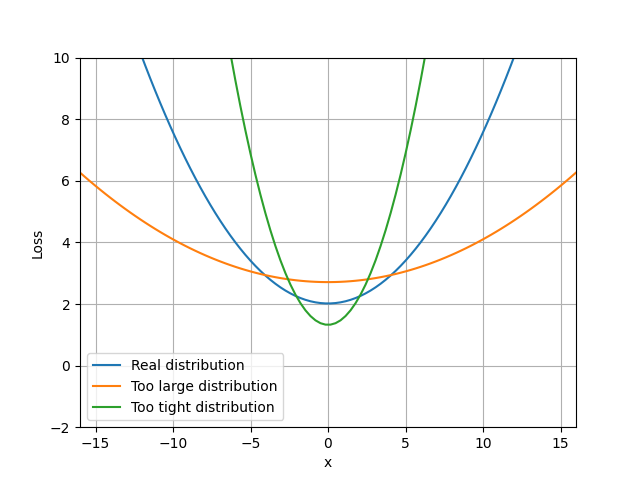
\includegraphics[width=400px]{distribution_comp.png}
    \caption{Comparison of the loss for a perfectly predicted distribution, a too large predicted distribution and a too tight distribution, with x the difference between the observed value and the median of the predicted distribution}
    \label{fig:distrib_comp}
\end{figure}


\subsection{Metrics} \label{metrics}

Concerning the evaluation of the results, GluonTS provides a module using the trained model and testing data to provide quantitative results, as metrics ("Aggregate", for all time series, or "Item", for each series separately). Metrics proposed by GluonTS includes \textit{MSE, MSIS, RMSE}, and other classical measures.

All metric function takes as argument \textit{N} randomly drawn sample values of the predicted probability distribution ($[{x_1},...,{x_N}]$) and one observed value y. 
For example the MSE metric function is defined as :
\begin{equation}
    MSE(y,[{x_1},...,{x_N}]) = \frac{1}{N}\sum_{i=0}^{N}(y-{x_i})^2
\end{equation}

"Item" metric value is the mean of metric value for each time step of the prediction window.
"Aggregate" metric value is the mean of "Item" metrics values for each time series.

In chapter \ref{part3}, as we use the default loss, metric function must correspond to this loss function, as it has been defined in section \ref{loss}. 

The problem is that the metric function cannot be equivalent to loss function, as these are functions with different inputs, the loss function taking as input the predicted distribution instead of randomly drawn point sample.
Nowadays, in fine, metrics like \textit{MSE, MSIS, RMSE} expresses the same goal than the log-negative likelihood of the loss function, i.e. the minimization of the difference between predicted and real distribution.
A high value of one of these metrics is proportional to a high value of the loss.
The metric chosen for the first model comparison in chapter \ref{part3} is \textit{MSE}.



\subsection{Distribution}\label{distribution}

GluonTs proposes different types of output distribution. In most of the models the output is technically
 a vector of values which is
transformed to a vector of distribution parameters  and put in a distribution object.
In current implementation, three different output distribution are functional. $Gaussian$, $Laplace$ and $PiecewiseLinear$.
$Student$ has been rejected because the quantiles of the distribution are not obtainable.
$Uniform$ has been rejected because of loss problems in execution.
Other options are available, as multiple kernel gaussian.
The GluonTS models are mandatory to output an object containing point sample of the distribution, not the distribution itself (parameters values). Considering that the parameter information could also be useful, as asked by the client, a modification done in custom models allows saving these information.

\begin{figure}[H]
    \centering
    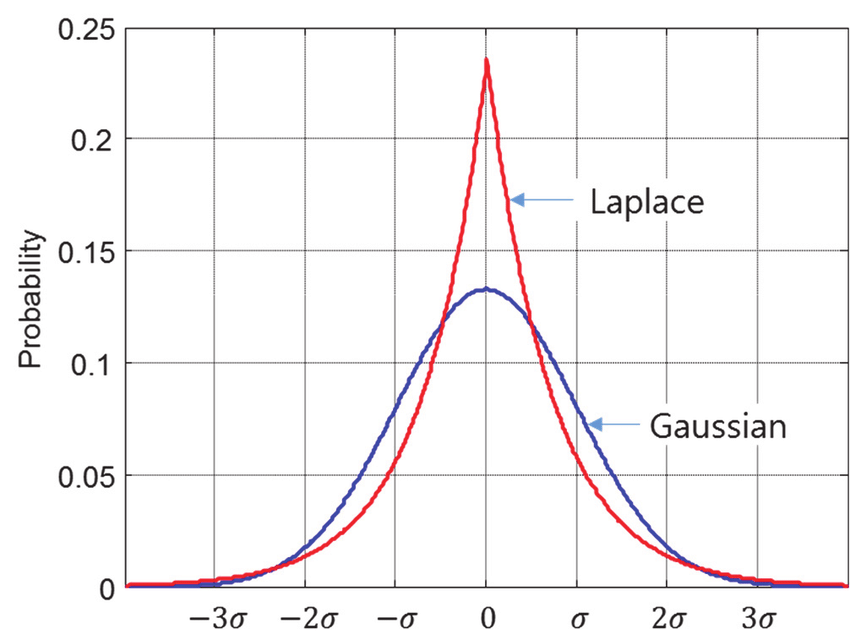
\includegraphics[width=200px]{Gaussian-distribution-and-Laplace-distribution.ppm.png}
    \caption{Comparison between Gaussian distribution and Laplace distribution}
    \label{fig:gausslaplace}
\end{figure}

\begin{figure}[H]
    \centering
    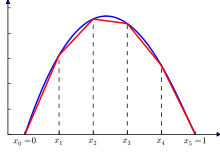
\includegraphics[width=200px]{220px-Finite_element_method_1D_illustration1.svg.png}
    \caption{Comparison between Gaussian distribution and PiecewiseLinear distribution}
    \label{fig:gausslaplace}
\end{figure}

\subsection{Models presentation} \label{diff_models}


All the pre-implemented deep learning models that have been tested  are presented here.
The models individual hyperparameters are mentioned in corresponding section.
The results for different values of hyperparameters are studied in section \ref{comp_model_param}.


\subsubsection{Simple} \label{descr_simple}
A manually implemented model which uses a simple 2 fully connected layers neural network.
The individual hyperparameter is the number of cells in layers.

\subsubsection{FeedForward} \label{descr_feedfordward}
A MLP (multi-layer perceptron) model.
The individual hyperparameter is the number of hidden nodes in each layer.

\subsubsection{Recurrent Neural Network} \label{descr_canonicalRNN}
A model which uses a recurrent neural network \ref{rnn_paper}.
The individual hyperparameters are the number of layers and number of cells of the network

\subsubsection{DeepAr} \label{descr_deepar}
Implementation of DeepAr estimator, a RNN based model, close to the one described in paper 
\textit{"DeepAR: Probabilistic Forecasting with Autoregressive Recurrent Networks"} \cite{deepar_paper}.
The individual hyperparameters are the same than for CanonicalRNN.

\subsubsection{Deep Factors} \label{descr_deepfactor}
Implementation of the 2019 ICML paper \textit{“Deep Factors for Forecasting”} \cite{deepar_factor}.
Uses a global RNN model to learn patterns across multiple related time series and an arbitrary local model to model the time series on a per time series basis. 
In the current implementation, the local model is a RNN (DF-RNN).
The individual hyperparameters are the number of units per hidden layers and the number of layers in the global model, the number of units and layers in the local model (not studied)
, the number of global factors.

\subsubsection{Gaussian Process} \label{descr_gp}
Model using Gaussian Processes (GP) \cite{gp_paper}.
Each time series has a GP with its own hyper parameters.
There are no hyperparameters to tune.

\subsubsection{NPTS} \label{descr_npts}
Implementation of the Non-Parametric Time Series Forecaster \cite{npts_paper}, 
which falls into the class of simple forecasters that use one of the past observed targets as the forecast for
the current time step. It randomly samples a past time index as the prediction for the time step T (auto regressive model, which predict step by step).
There are no hyperparameters to tune, but it exists some variants.

\subsubsection{MQCNN} \label{descr_mqcnn}
Discriminative Sequence to Sequence model constructed using the \textit{SeqtoSeq} framework of GluonTS to reproduce the model of the 
paper \textit{"A Multi-Horizon Quantile Recurrent Forecaster"}\cite{mqcnn_paper}.
Sequence to sequence models are composed of two parts. The encoder network, that reads the training window of the time series 
and encodes information about  the  sequence  in  a  latent  state.
And the decoder network, which generates the forecast by combining the latent information with the features in the prediction range.
In MQCNN, the encoder is a Convolutionnal Neural Network and the decoder an MLP. Unlike other presented models, the output is not technically a distribution but the quantiles itself, that are point predicted values obtains by optimizing the corresponding quantile loss.
The individual hyperparameter is the  dimension of the MLP decoder.
Considering the fundamental difference in the intern functioning, it not seems to be possible to modify the loss, see discussion in \ref{custom_loss} section.

\subsubsection{MQRNN} \label{descr_mqrnn}
Same as MQCNN but with a Recurrent Neural Network encoder instead.

\subsection{Others}

Other models, recently added to GluonTS,  will be added. At least 3 (Wavenet, DeepVar, NBEATS)


\section{First Models Comparison}
\label{part3}

\subsection{Testing protocol definition}


Each comparison is presented using as element of comparison the metric \textit{MSE}, as defined in section \ref{metrics}.
The models uses the default loss as defined in section \ref{loss}

The plot results are all presented with the same values of quantiles, the quantile $quantile(0.99)$ and the respective $quantile(0.01)$ but also the $quantile(0.9)$, $quantile(0.1)$ and the median.
Before the comparison between different models, we need to compare the impact of the values of the different hyperparameters of the problem.
The hyperparameters of the problem are :
\begin{itemize}
    \item The size of time series
    \item The learning rate of the model training
    \item The number of epochs of the training
    \item The output distribution, defined in section \ref{distribution}
    \item The individual hyperparameters of the different models
\end{itemize}
Each comparison section is interested in one particular hyperparameter of the problem.
In general the other hyperparameters takes default values, as given by GluonTS.

\subsection{Global Hyperparameters comparison}

\subsubsection{Different dataset configurations}

There is no quantitative comparison to do, considering that the goal is not to find the configuration which gives the better results. The quantitative results are not significant, except noticing that the results are indeed influenced by the configuration. 
In general the following section will consider configuration A as default, but if necessary other configuration will be tested.

\subsubsection{Time series size} \label{comp_lr}

\begin{figure}[H]
    \centering
    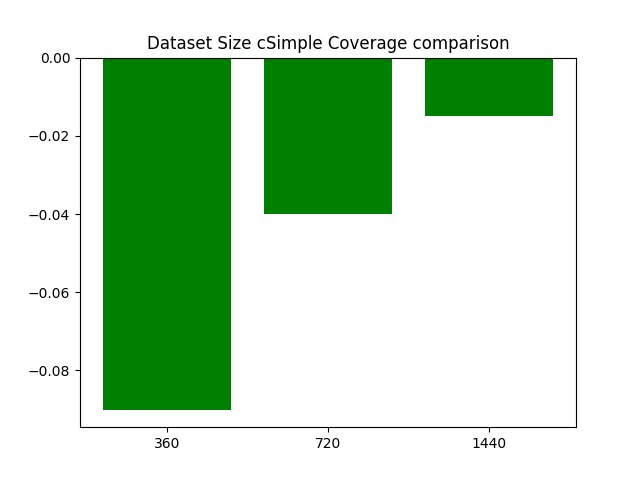
\includegraphics[width=300px]{plots/hist/a/datasize/cSimple/Coverage.png}
    %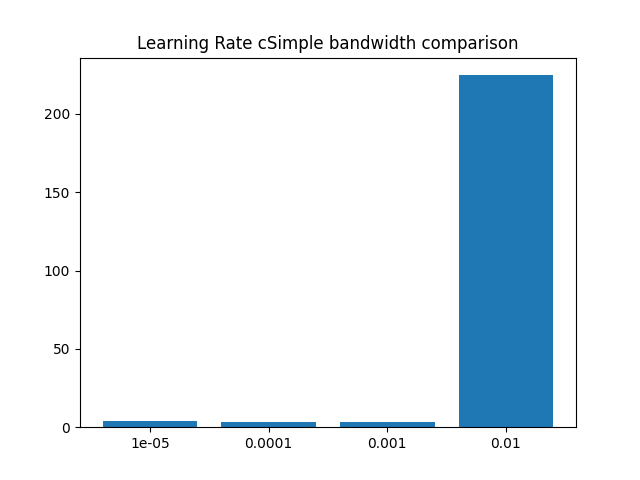
\includegraphics[width=200px]{plots/hist/a/lr/cSimple/bandwidth.png}
    %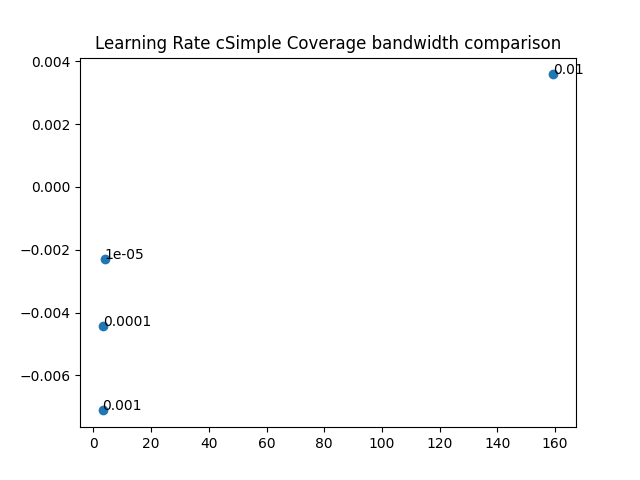
\includegraphics[width=300px]{plots/scatter/a/lr/cSimple/Coverage_bandwidth.png}
    \caption{Comparison of different time series size (Model: Simple (Default parameter values), Epochs = 100, $\alpha$ = 0.9, Distribution = Gaussian, Config A)}
    \label{fig:comp_datasize}
\end{figure}


\subsubsection{Learning rate} \label{comp_lr}

\begin{figure}[H]
    \centering
    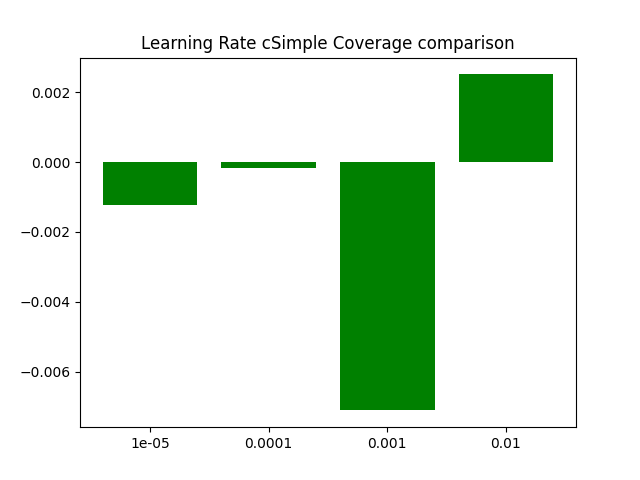
\includegraphics[width=300px]{plots/hist/a/lr/cSimple/Coverage.png}
    %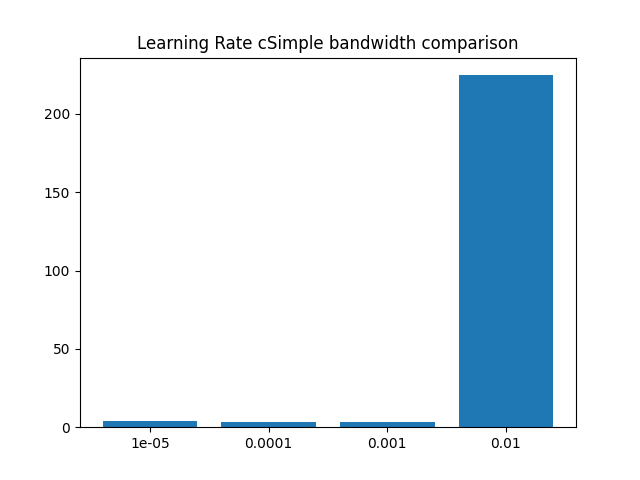
\includegraphics[width=200px]{plots/hist/a/lr/cSimple/bandwidth.png}
    %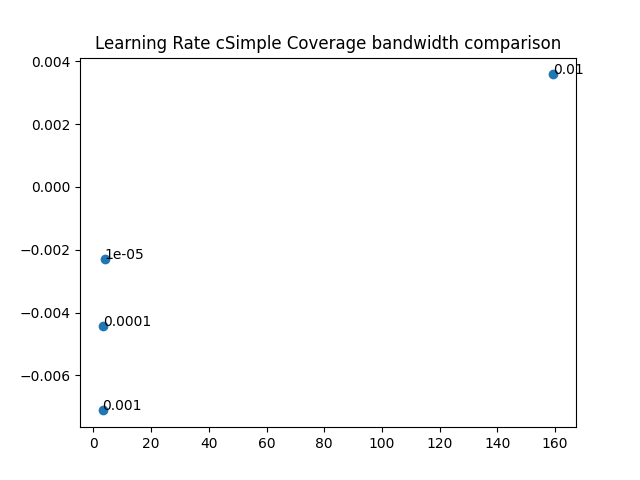
\includegraphics[width=300px]{plots/scatter/a/lr/cSimple/Coverage_bandwidth.png}
    \caption{Comparison of different learning rate (Model: Simple (Default parameter values), Epochs = 100, $\alpha$ = 0.9, Distribution = Gaussian, Config A)}
    \label{fig:comp_lr}
\end{figure}

The default learning rate in GluonTs for all deep learning models is $1^{-3}$
Learning rate as a great impact on the results.

\subsubsection{Epochs} \label{comp_epochs}

\begin{figure}[H]
    \centering
    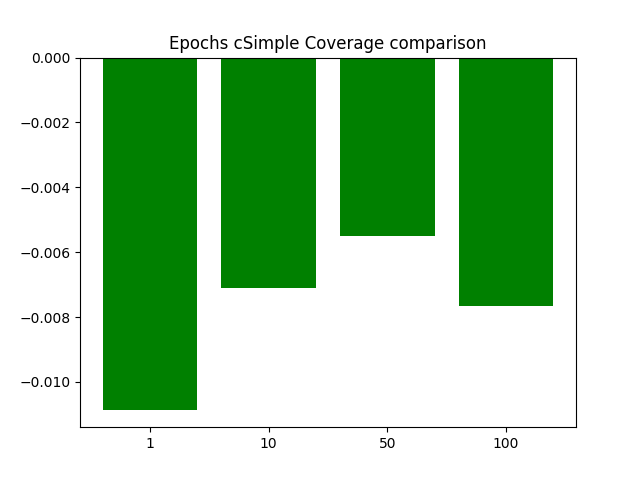
\includegraphics[width=300px]{plots/hist/a/epochs/cSimple/Coverage.png}
    %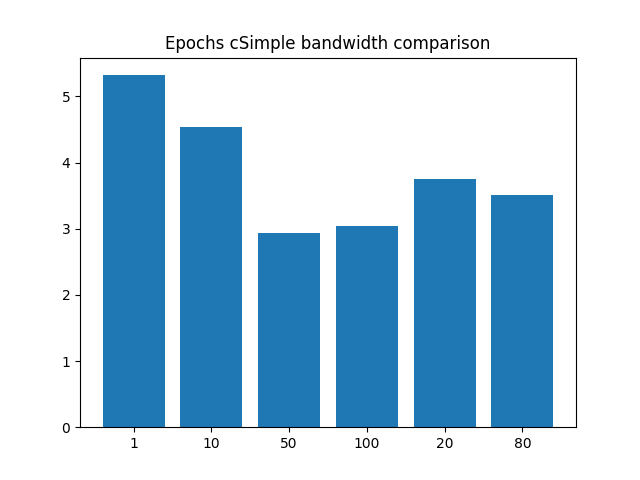
\includegraphics[width=200px]{plots/hist/a/epochs/cSimple/bandwidth.png}
    %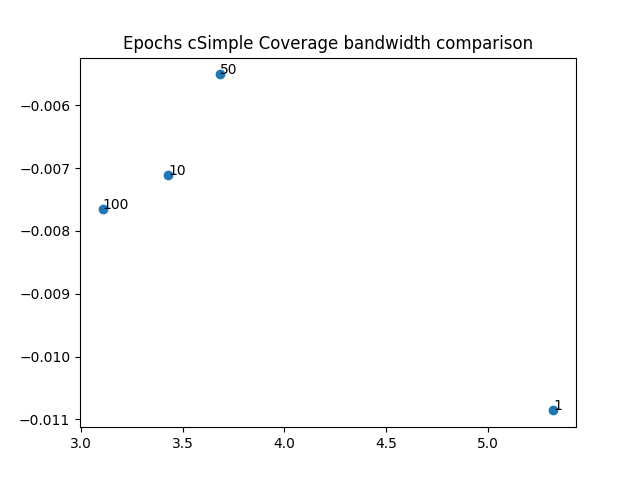
\includegraphics[width=300px]{plots/scatter/a/epochs/cSimple/Coverage_bandwidth.png}
    \caption{Comparison of different epochs number (Model: Simple (Default parameter values), $\alpha$ = 0.9, Distribution = Gaussian, Config A)}
    \label{fig:comp_epochs}
\end{figure}

All the deep learning models implemented must be trained a certain number of epochs. The default number 
is 100 epochs. This value is a good choice (better bandwidth of the comparison), as are values slightly  inferior (which have better Coverage). 

\newpage

\subsubsection{Output Distribution} \label{comp_outdistrib}

\begin{figure}[H]
    \centering
    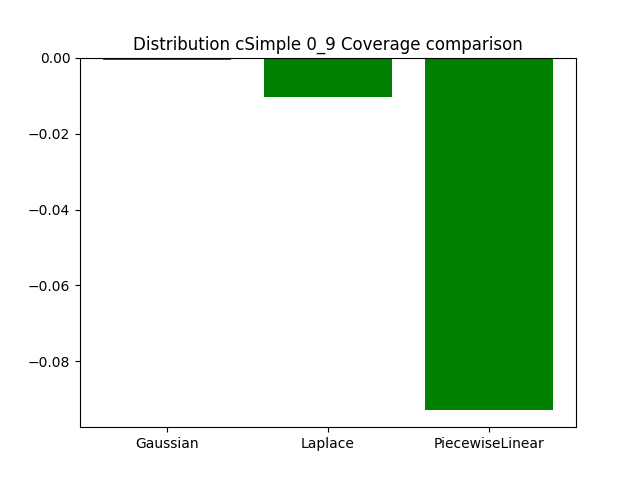
\includegraphics[width=300px]{plots/hist/a/distribution/cSimple/0_9/Coverage.png}
    %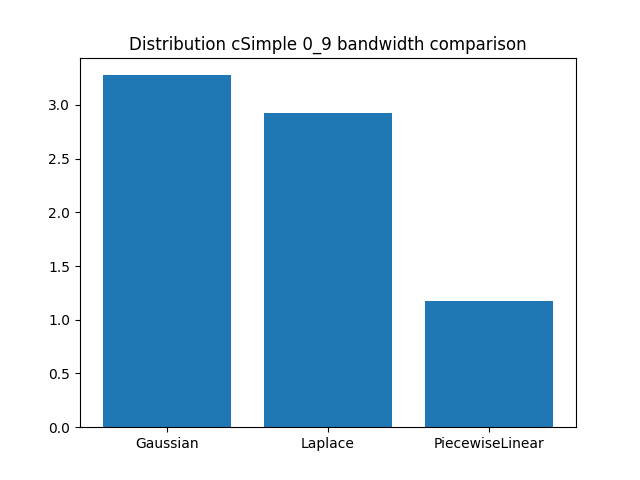
\includegraphics[width=200px]{plots/hist/a/distribution/cSimple/0_9/bandwidth.png}
    %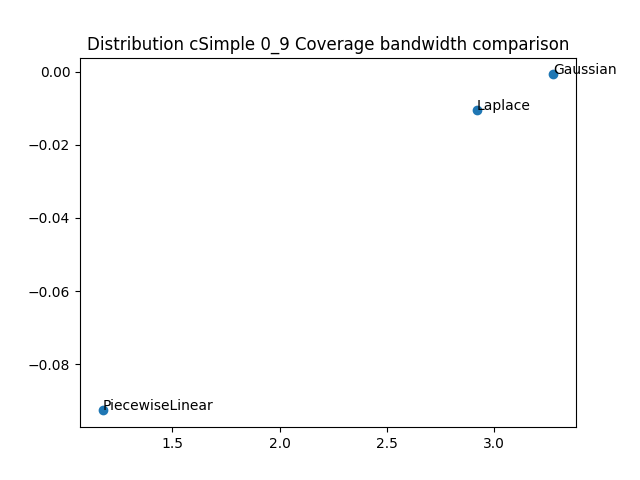
\includegraphics[width=300px]{plots/scatter/a/distribution/cSimple/0_9/Coverage_bandwidth.png}
    \caption{Comparison of different output distribution (Model: Simple (Default parameter values), Epochs = 100, $\alpha$ = 0.9,  Config A)}
    \label{fig:comp_outdistrib}
\end{figure}

% \textit{PiecewiseLinear} distribution gives very thin distribution but clearly underestimate the risk, and would be not chosen in consequence. Laplace gives slightly better results than Gaussian if we consider Coverage and bandwith as the same level of importance. 


\subsection{Different models parameters comparison and results} \label{comp_model_param}

The different models are described in the \ref{diff_models} section

\subsubsection{Simple} \label{comp_simple}

\begin{figure}[H]
    \centering
    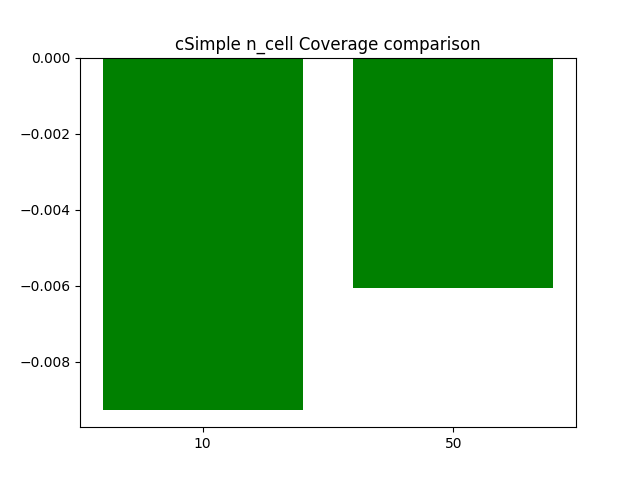
\includegraphics[width=300px]{plots/hist/a/cSimple/n_cell/Coverage.png}
    %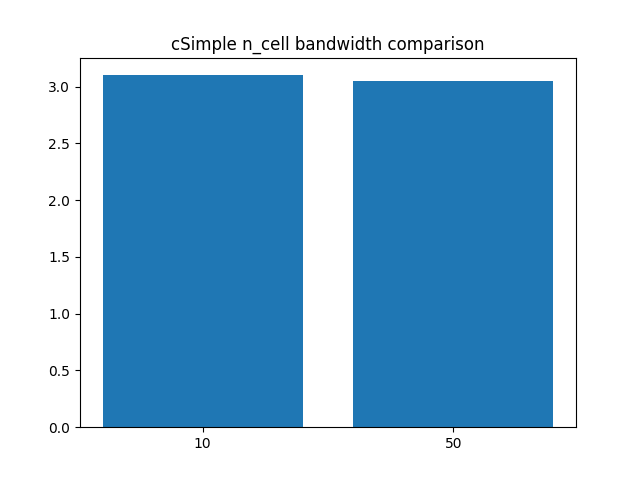
\includegraphics[width=200px]{plots/hist/a/cSimple/n_cell/bandwidth.png}
    %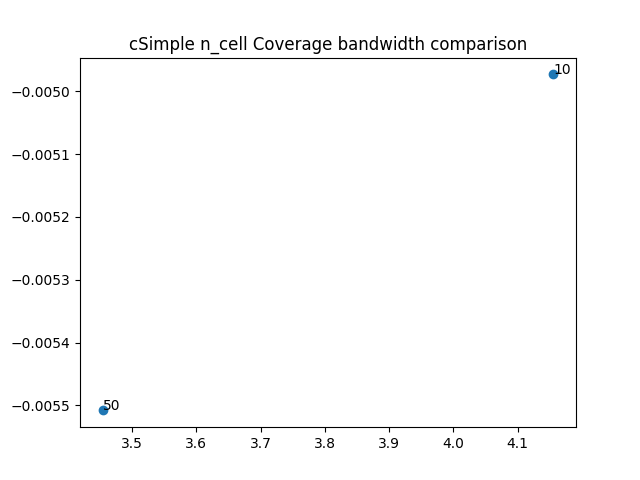
\includegraphics[width=300px]{plots/scatter/a/cSimple/n_cell/Coverage_bandwidth.png}
    \caption{Comparison of different $n\_cell$ values for Simple model (Epochs = 100, Distribution = Gaussian, $\alpha = 0.9$, Config A)}
    \label{fig:comp_simple}
\end{figure}

\begin{figure}[H]
    \centering
    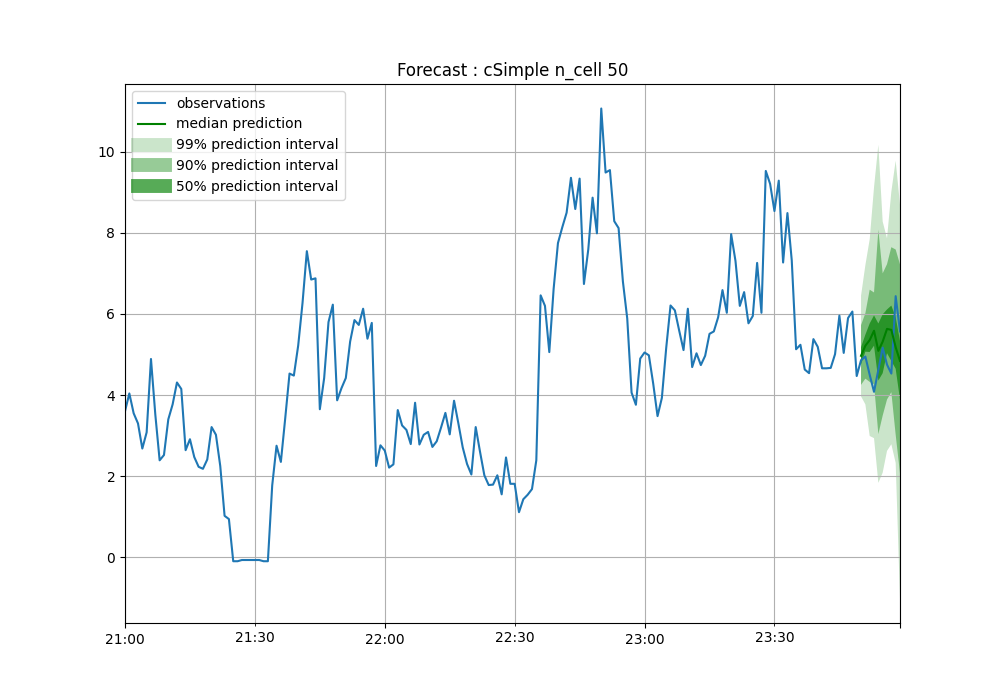
\includegraphics[width=400px]{plots/forecast/a/cSimple/n_cell/50/180.png}
    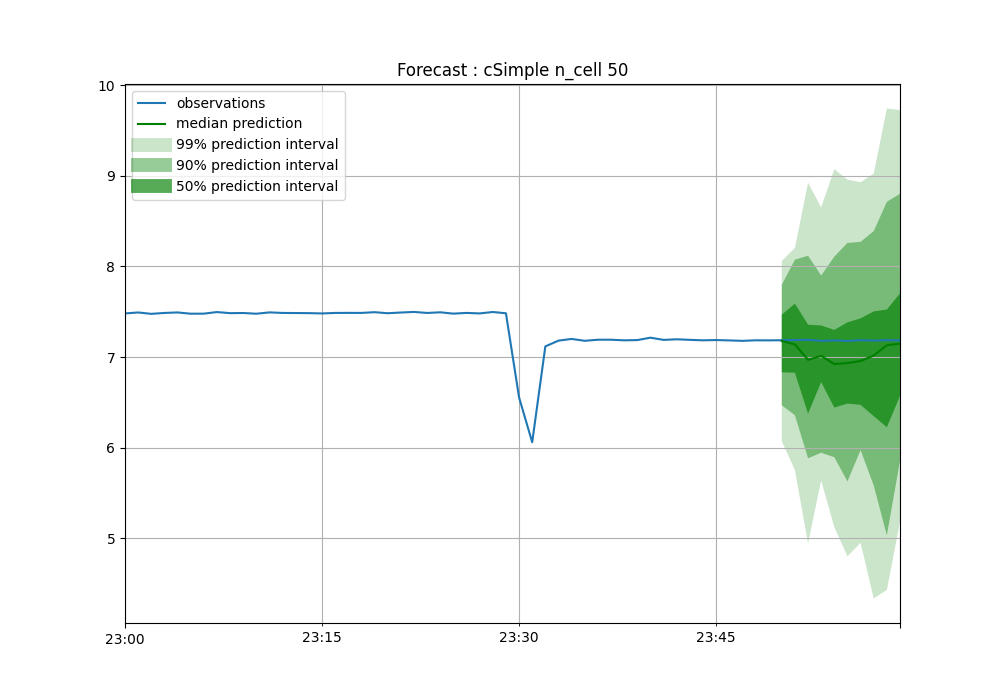
\includegraphics[width=400px]{plots/forecast/a/cSimple/n_cell/50/60.png}
    \caption{Forecast result of Simple model at 3 hours and 1 hour scale ($n\_cell = 50$ Epochs = 100, Distribution = Gaussian, $\alpha = 0.9$, Config A)}
    \label{fig:simple}
\end{figure}


\subsubsection{Simple Feed Fordward} \label{comp_feedfordward}

\begin{figure}[H]
    \centering
    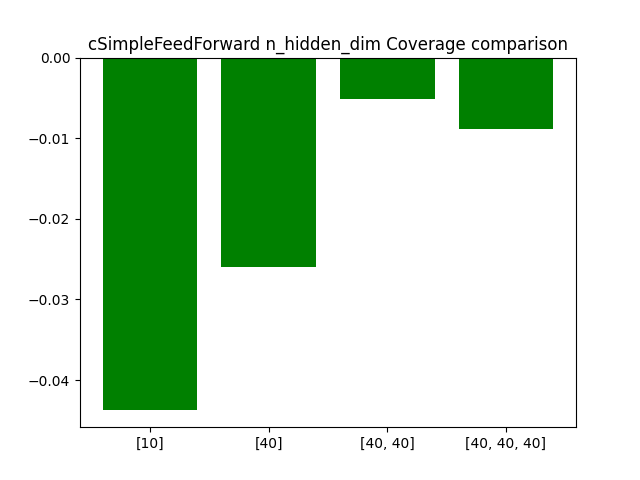
\includegraphics[width=300px]{plots/hist/a/cSimpleFeedForward/n_hidden_dim/Coverage.png}
    %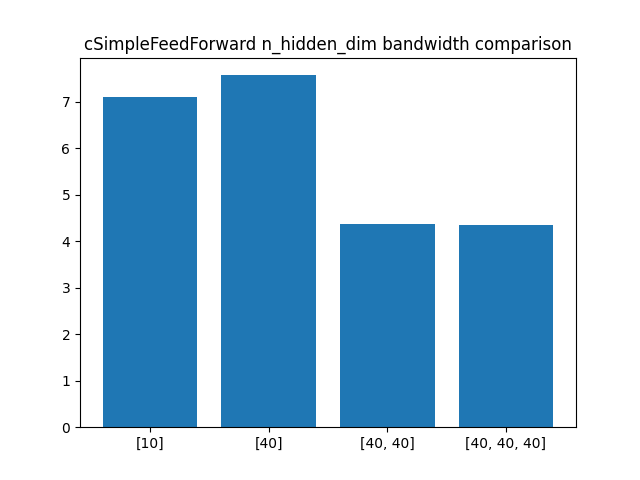
\includegraphics[width=200px]{plots/hist/a/cSimpleFeedForward/n_hidden_dim/bandwidth.png}
    %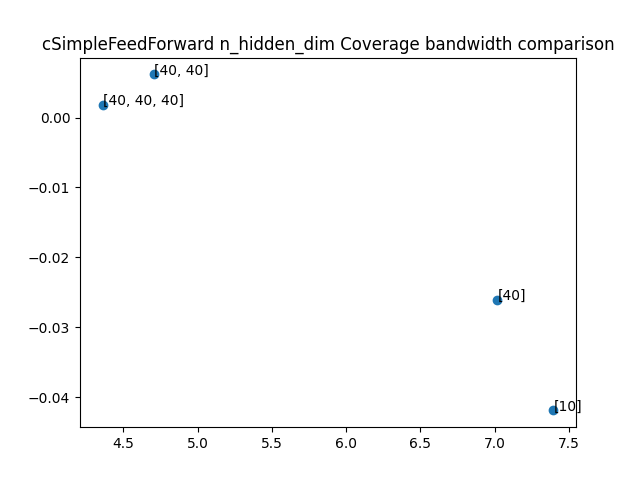
\includegraphics[width=300px]{plots/scatter/a/cSimpleFeedForward/n_hidden_dim/Coverage_bandwidth.png}
    \caption{Comparison of different $n\_hidden\_dim$ values for Simple FeedForward model (Epochs = 100, Distribution = Gaussian, $\alpha = 0.9$, Config A)}
    \label{fig:comp_feedfordward}
\end{figure}

\begin{figure}[H]
    \centering
    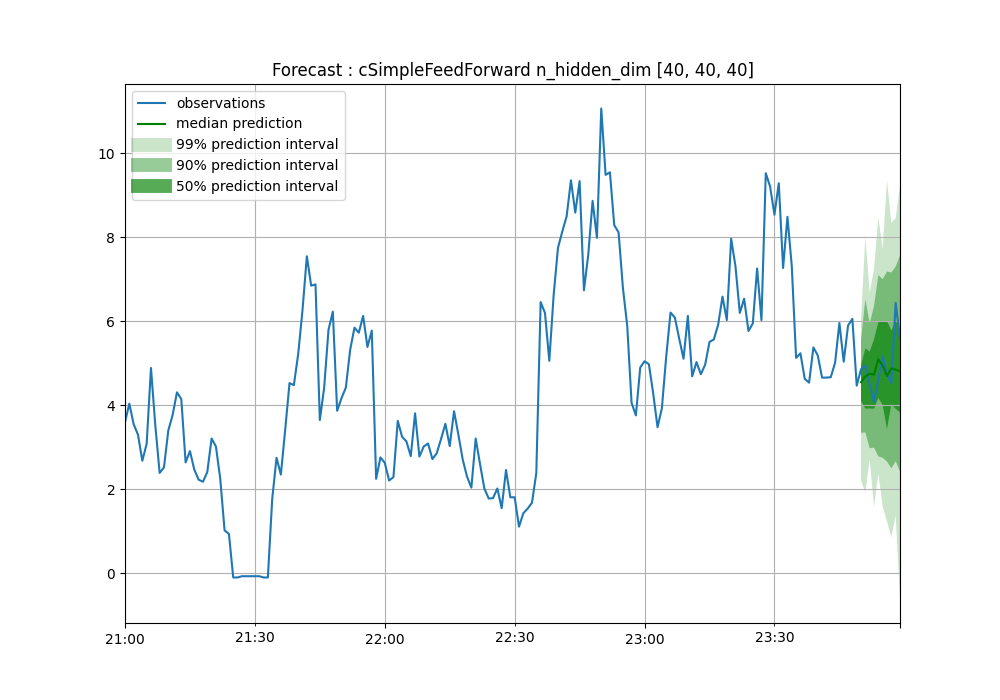
\includegraphics[width=400px]{plots/forecast/a/cSimpleFeedForward/n_hidden_dim/[40, 40, 40]/180.png}
    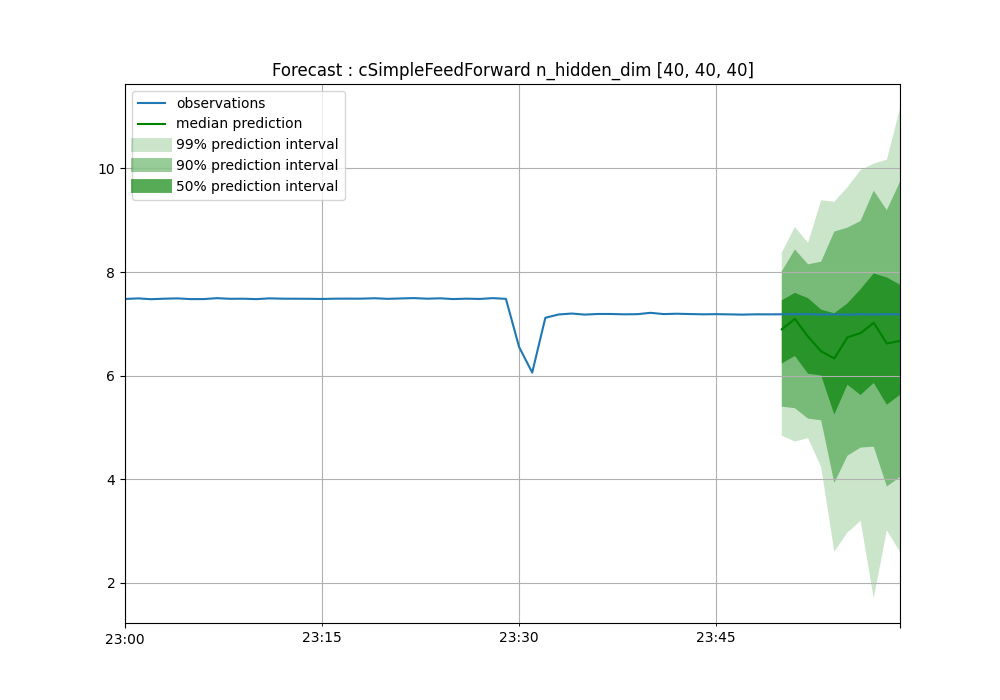
\includegraphics[width=400px]{plots/forecast/a/cSimpleFeedForward/n_hidden_dim/[40, 40, 40]/60.png}
    \caption{Forecast result of Simple FeedForward model at 3 hours and 1 hour scale ($n\_hidden_dim = [40,40,40]$ Epochs = 100, Distribution = Gaussian, $\alpha = 0.9$, Config A)}
    \label{fig:feedfordward}
\end{figure}


\subsubsection{Canonical RNN} \label{comp_canonicalrnn}

\begin{figure}[H]
    \centering
    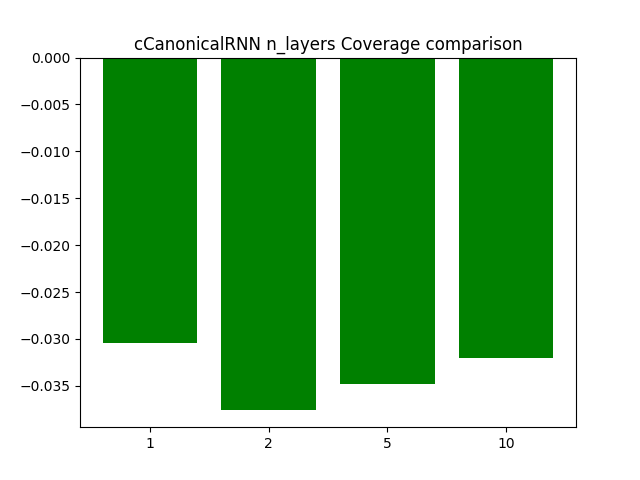
\includegraphics[width=300px]{plots/hist/a/cCanonicalRNN/n_layers/Coverage.png}
    %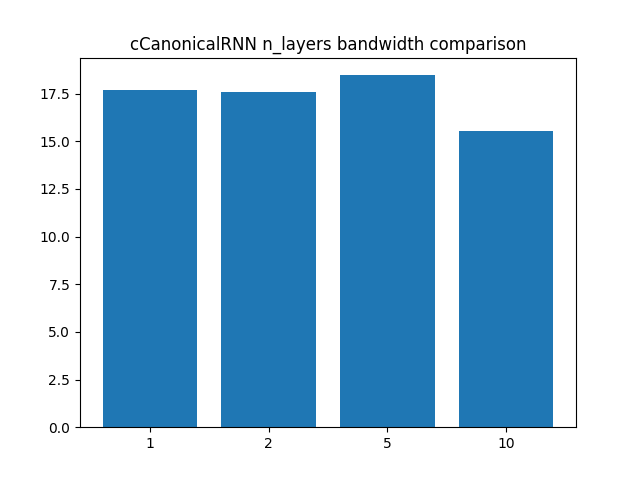
\includegraphics[width=200px]{plots/hist/a/cCanonicalRNN/n_layers/bandwidth.png}
    %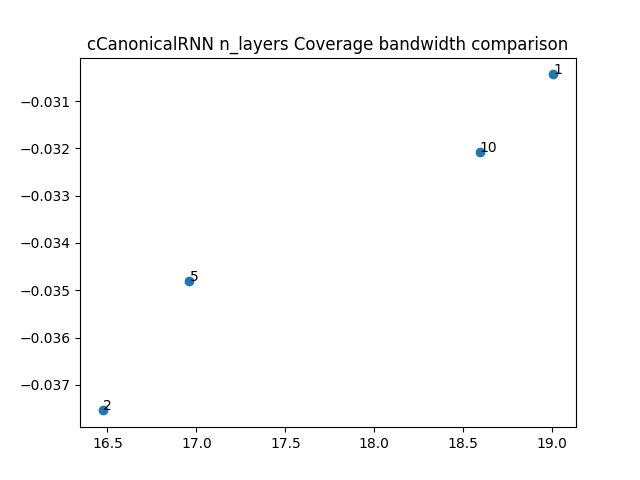
\includegraphics[width=300px]{plots/scatter/a/cCanonicalRNN/n_layers/Coverage_bandwidth.png}
    \caption{Comparison of different $n\_layers$ values for Canonical RNN model (Epochs = 100, Distribution = Gaussian, $\alpha = 0.9$, Config A)}
    \label{fig:comp_canonicalrnn}
\end{figure}

\begin{figure}[H]
    \centering
    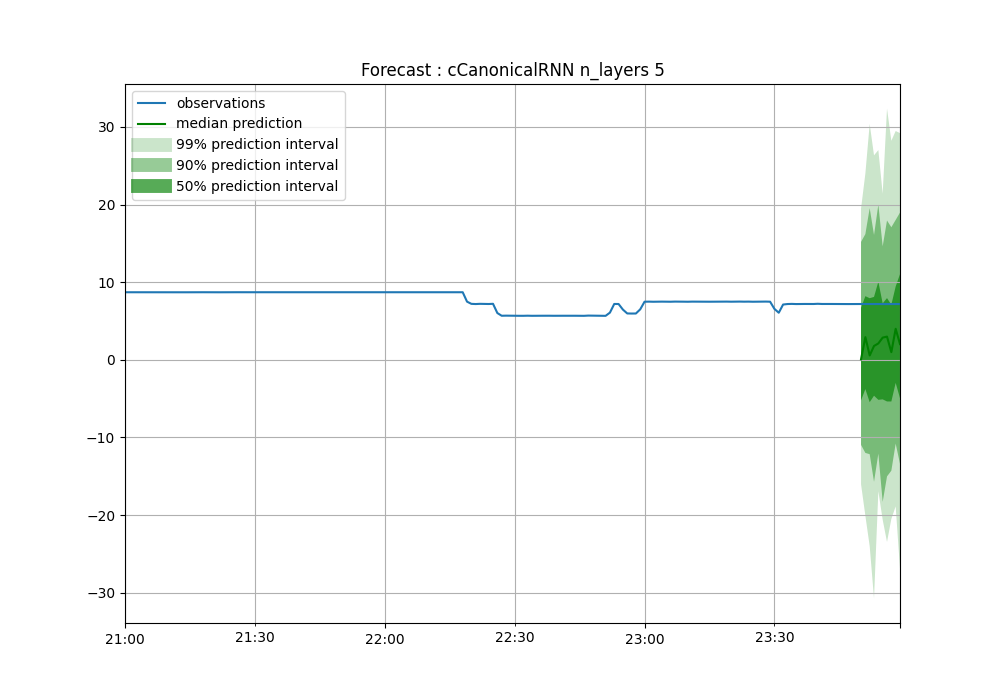
\includegraphics[width=400px]{plots/forecast/a/cCanonicalRNN/n_layers/5/180.png}
    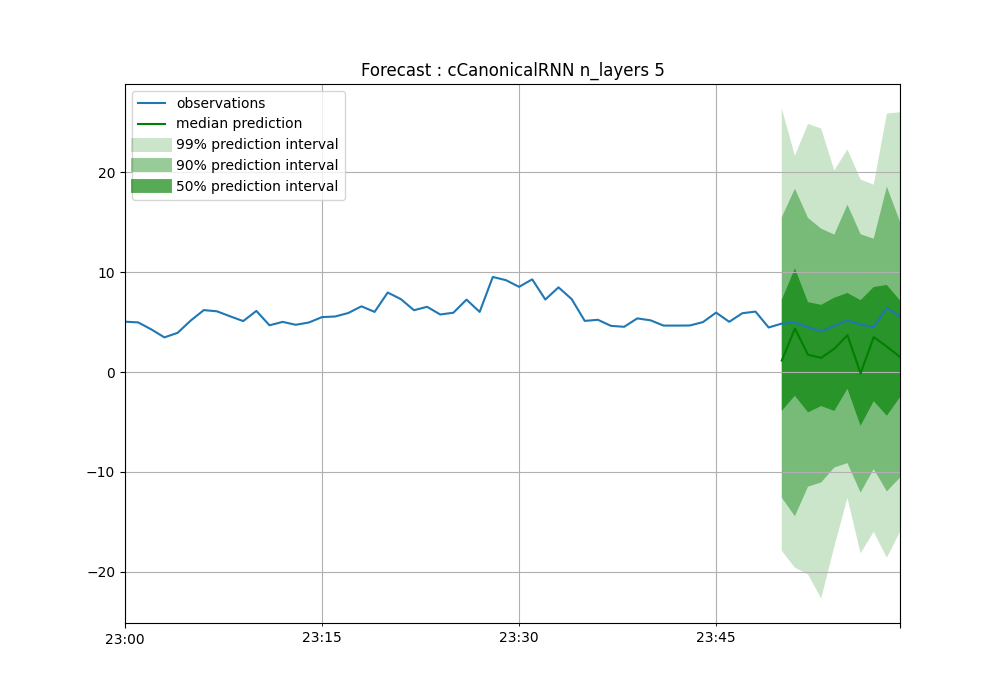
\includegraphics[width=400px]{plots/forecast/a/cCanonicalRNN/n_layers/5/60.png}
    \caption{Forecast result of Simple FeedForward model at 3 hours and 1 hour scale ($n\_layers = 5$ Epochs = 100, Distribution = Gaussian, $\alpha = 0.9$, Config A)}
    \label{fig:canonicalrnn}
\end{figure}


\subsubsection{Deep AR} \label{comp_deepar}

\begin{figure}[H]
    \centering
    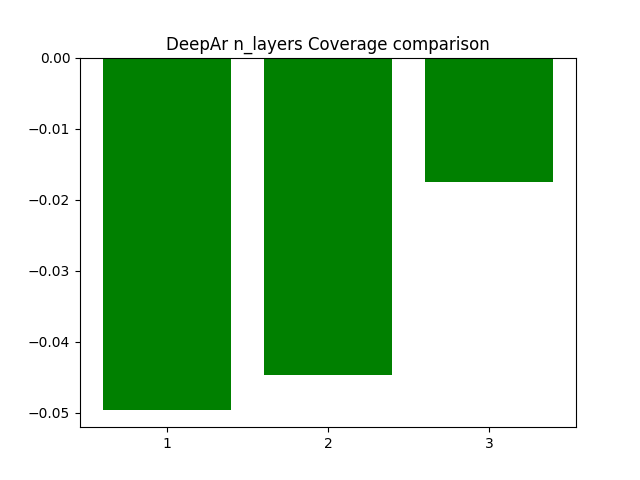
\includegraphics[width=300px]{plots/hist/a/DeepAr/n_layers/Coverage.png}
    %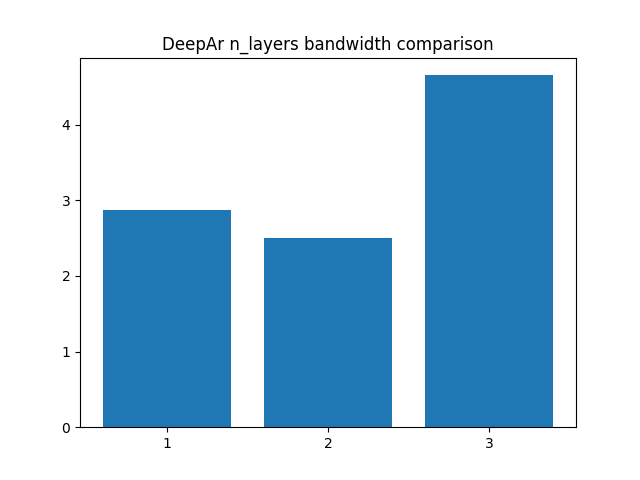
\includegraphics[width=200px]{plots/hist/a/DeepAr/n_layers/bandwidth.png}
    %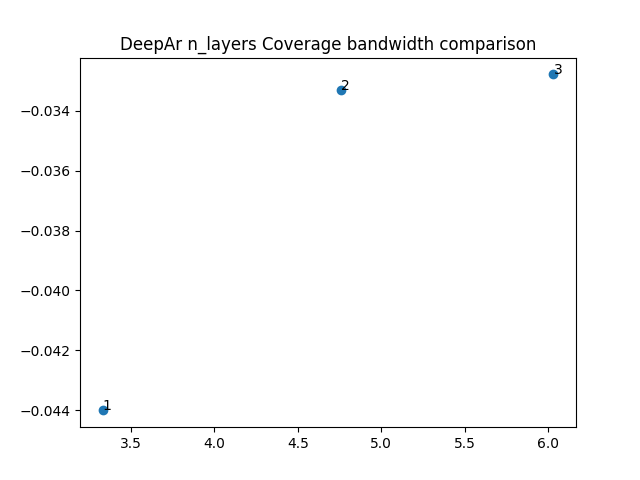
\includegraphics[width=300px]{plots/scatter/a/DeepAr/n_layers/Coverage_bandwidth.png}
    \caption{Comparison of different $n\_layers$ values for Deep AR model (Epochs = 100, Distribution = Gaussian, Config A)}
    \label{fig:comp_deepar_n_layers}
\end{figure}

\begin{figure}[H]
    \centering
    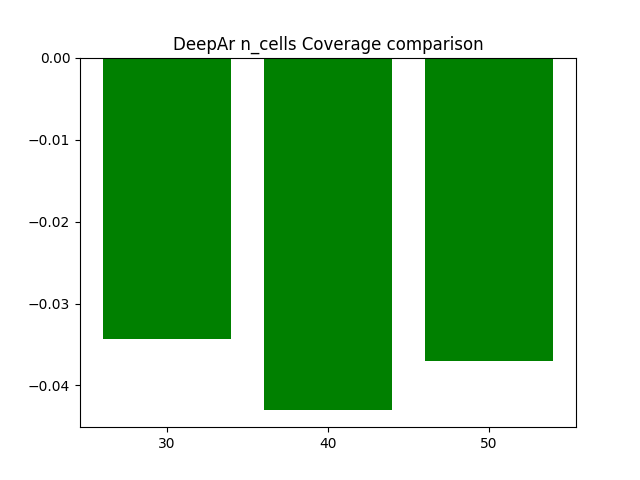
\includegraphics[width=300px]{plots/hist/a/DeepAr/n_cells/Coverage.png}
    %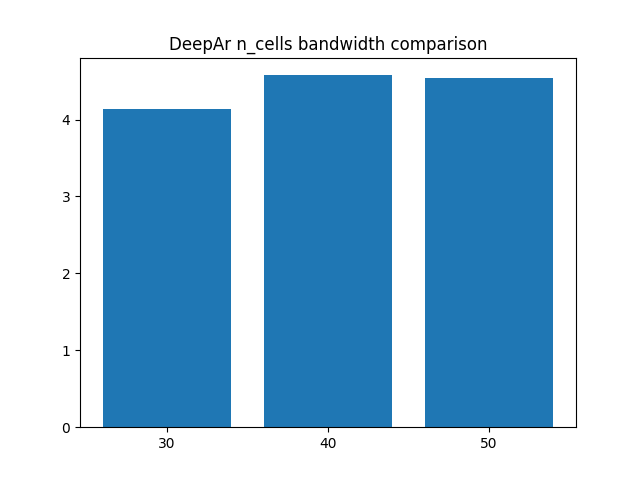
\includegraphics[width=200px]{plots/hist/a/DeepAr/n_cells/bandwidth.png}
    %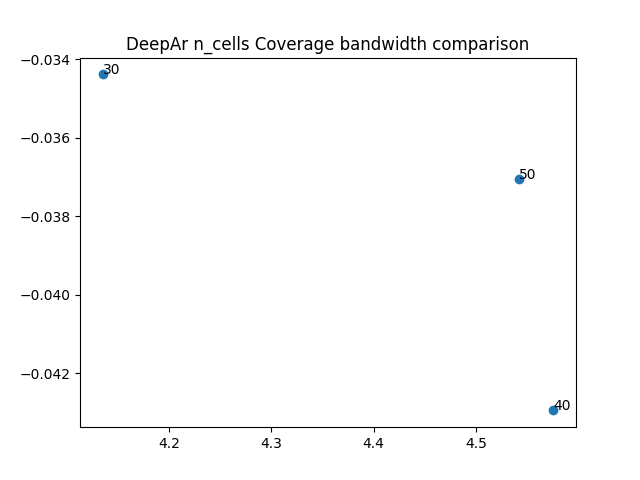
\includegraphics[width=300px]{plots/scatter/a/DeepAr/n_cells/Coverage_bandwidth.png}
    \caption{Comparison of different $n\_cells$ values for Deep AR model (Epochs = 100, Distribution = Gaussian, Config A)}
    \label{fig:comp_deepar_n_cells}
\end{figure}

\begin{figure}[H]
    \centering
    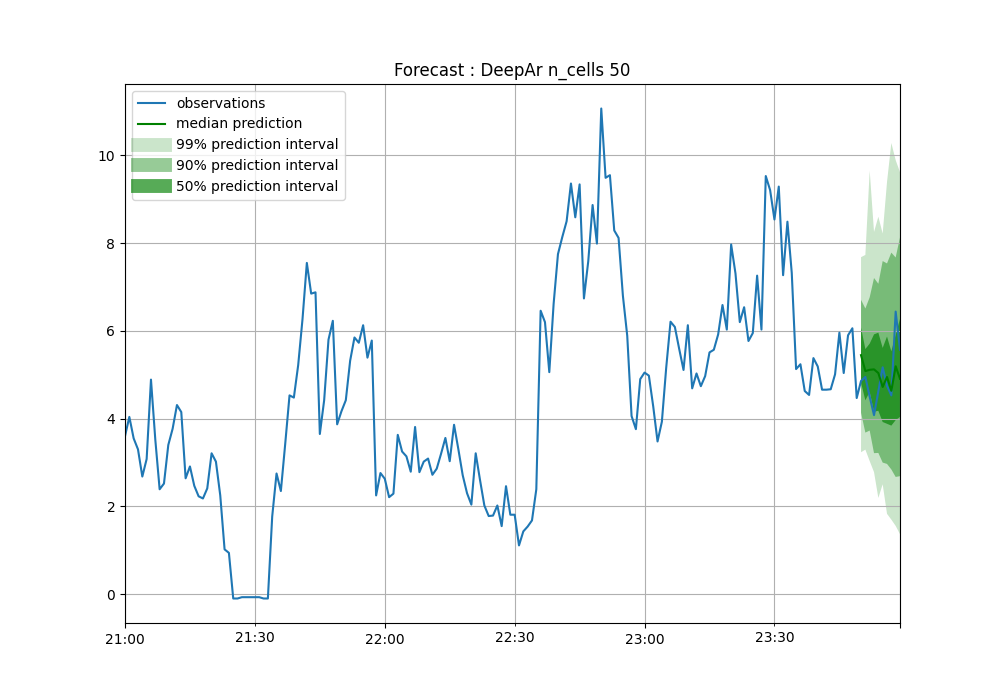
\includegraphics[width=400px]{plots/forecast/a/DeepAr/n_cells/50/180.png}
    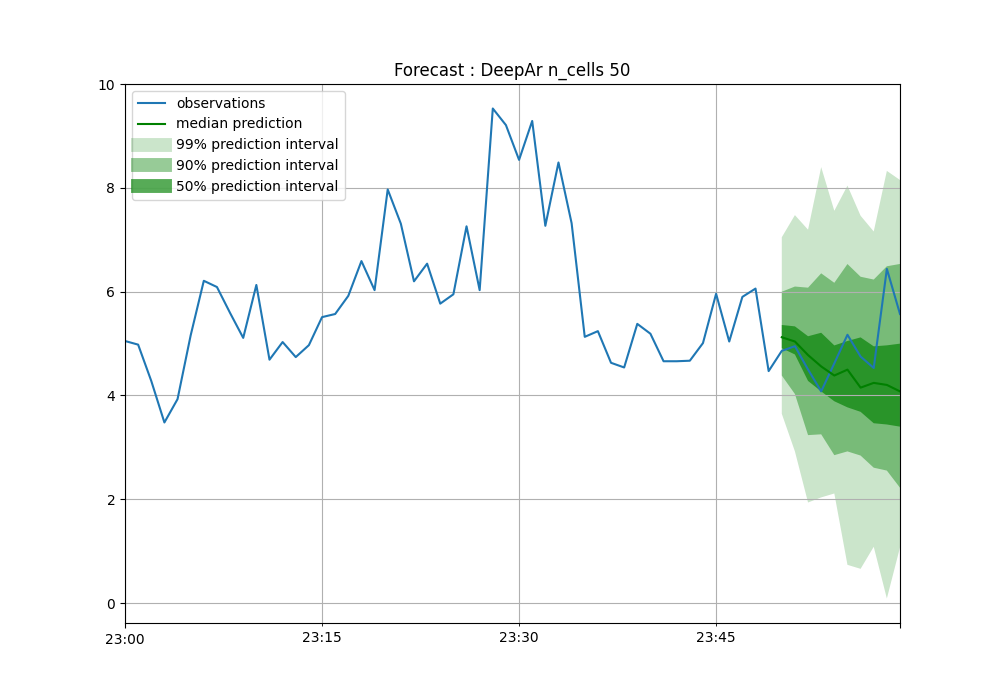
\includegraphics[width=400px]{plots/forecast/a/DeepAr/n_cells/50/60.png}
    \caption{Forecast result of Deep Ar model at 3 hours and 1 hour scale ($n\_layers = 2$, $n\_cells = 50$, Epochs = 100, Distribution = Gaussian, Config A)}
    \label{fig:deepar}
\end{figure}

\subsubsection{Deep Factor} \label{comp_deepfactor}

\begin{figure}[H]
    \centering
    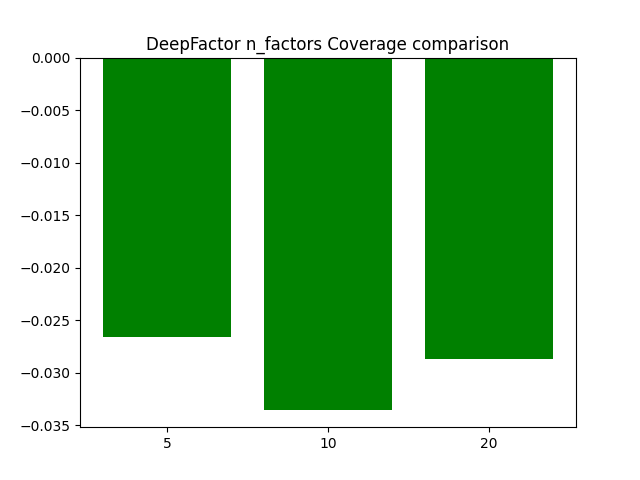
\includegraphics[width=300px]{plots/hist/a/DeepFactor/n_factors/Coverage.png}
    %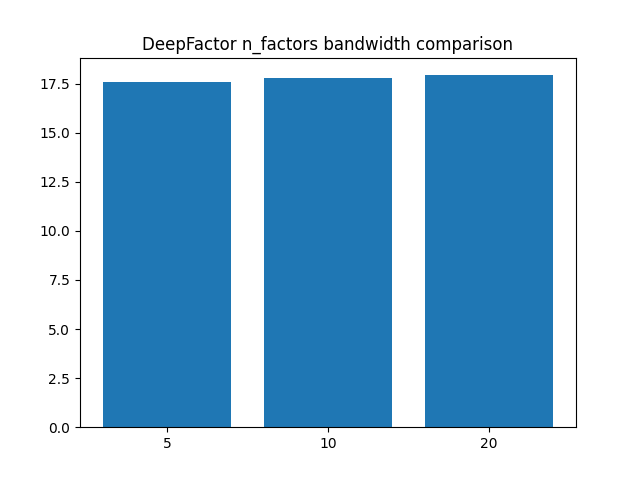
\includegraphics[width=200px]{plots/hist/a/DeepFactor/n_factors/bandwidth.png}
    %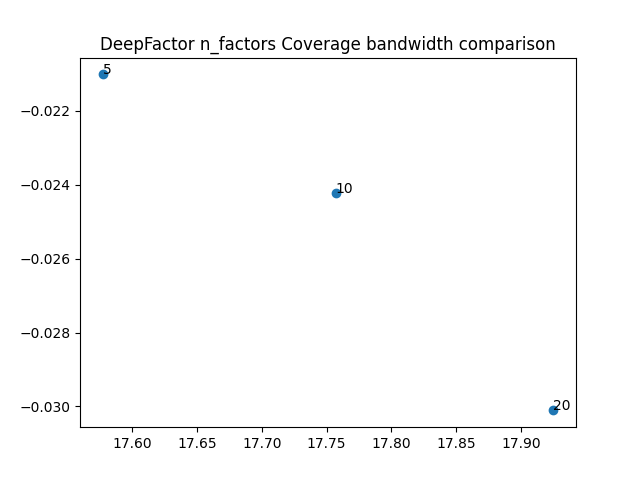
\includegraphics[width=300px]{plots/scatter/a/DeepFactor/n_factors/Coverage_bandwidth.png}
    \caption{Comparison of different $n\_factors$ values for Deep Factors model (Epochs = 100, Distribution = Gaussian, $\alpha = 0.9$, Config A)}
    \label{fig:comp_deepfactor_n_factors}
\end{figure}

\begin{figure}[H]
    \centering
    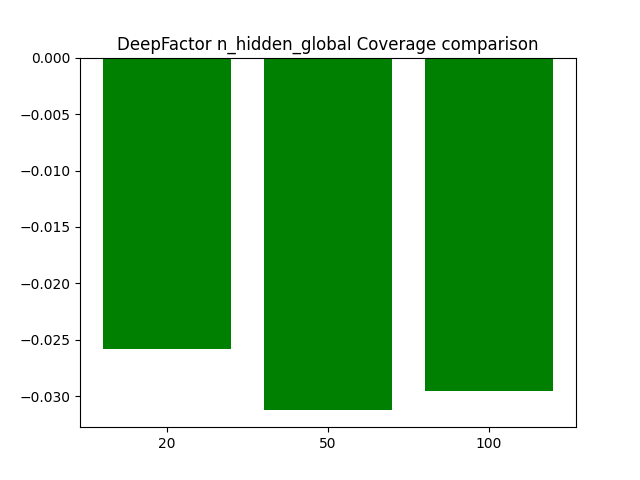
\includegraphics[width=300px]{plots/hist/a/DeepFactor/n_hidden_global/Coverage.png}
    %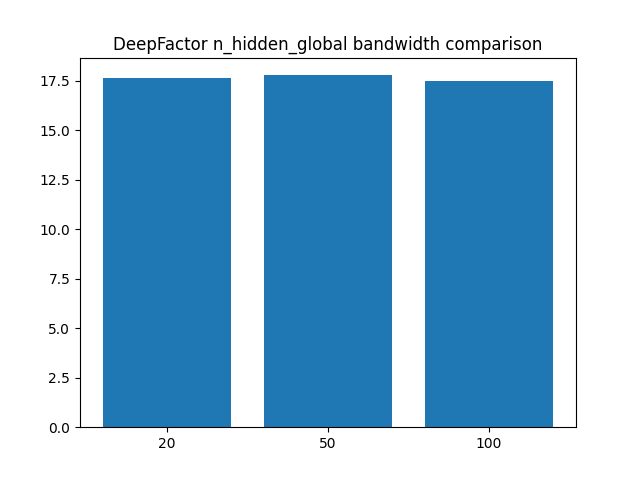
\includegraphics[width=200px]{plots/hist/a/DeepFactor/n_hidden_global/bandwidth.png}
    %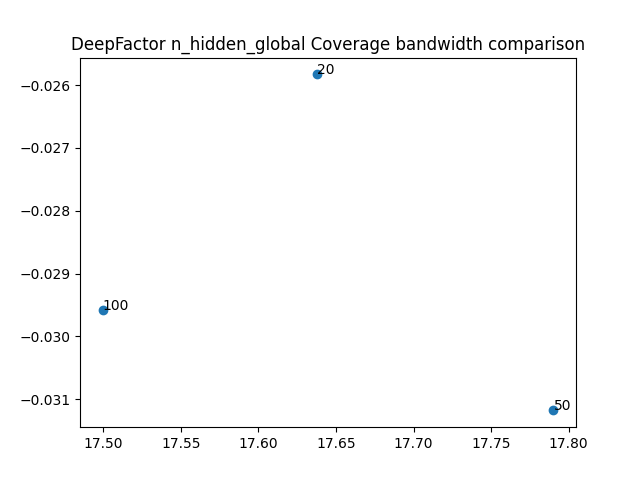
\includegraphics[width=300px]{plots/scatter/a/DeepFactor/n_hidden_global/Coverage_bandwidth.png}
    \caption{Comparison of different $n\_hidden\_global$ values for Deep Factors model (Epochs = 100, Distribution = Gaussian, $\alpha = 0.9$, Config A)}
    \label{fig:comp_deepfactor_n_hidden_globals}
\end{figure}

\begin{figure}[H]
    \centering
    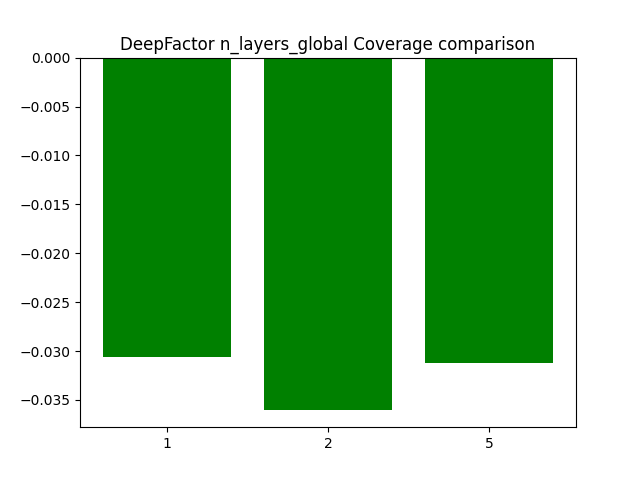
\includegraphics[width=300px]{plots/hist/a/DeepFactor/n_layers_global/Coverage.png}
    %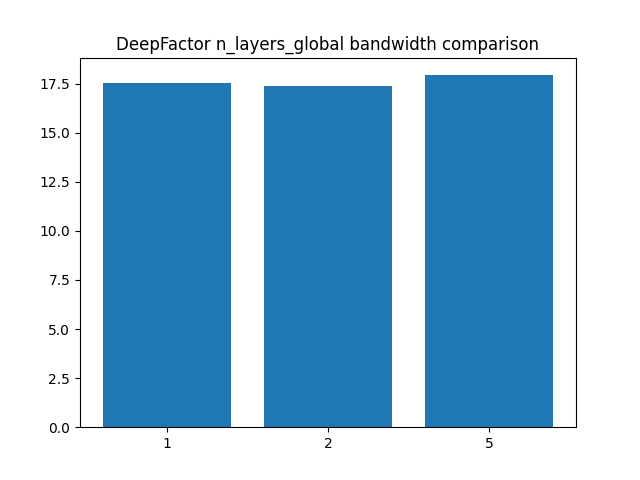
\includegraphics[width=200px]{plots/hist/a/DeepFactor/n_layers_global/bandwidth.png}
    %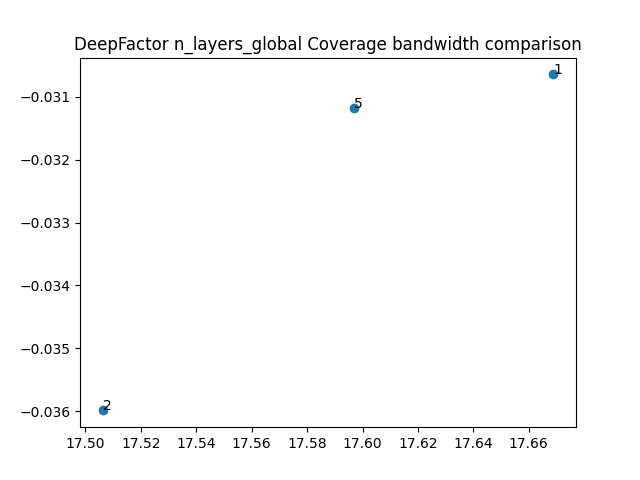
\includegraphics[width=300px]{plots/scatter/a/DeepFactor/n_layers_global/Coverage_bandwidth.png}
    \caption{Comparison of different $n\_layers\_global$ values for Deep Factors model (Epochs = 100, Distribution = Gaussian, $\alpha = 0.9$, Config A)}
    \label{fig:comp_deepfactor_n_layers_global}
\end{figure}

\begin{figure}[H]
    \centering
    \includegraphics[width=400px]{plots/forecast/a/DeepFactor/n_hidden_global/100/180.png}
    \includegraphics[width=400px]{plots/forecast/a/DeepFactor/n_hidden_global/100/60.png}
    \caption{Forecast result of Deep Factors model at 3 hours and 1 hour scale ($n\_factors = 5$, $n\_hidden\_global = 100$, $n\_layers\_global = 1$ Epochs = 100, Distribution = Gaussian, $\alpha = 0.9$, Config A)}
    \label{fig:comp_deepfactor_n_hidden_global}
\end{figure}

Contrary to another model, different hyperparameters of Deep Factors had a relatively low impact on the quality of the model.

\subsubsection{MQCNN} \label{comp_mqcnn}

\begin{figure}[H]
    \centering
    \includegraphics[width=300px]{plots/hist/a/MQCNN/mlp_final_dim/Coverage.png}
    %\includegraphics[width=200px]{plots/hist/a/MQCNN/mlp_final_dim/bandwidth.png}
    %\includegraphics[width=300px]{plots/scatter/a/MQCNN/mlp_final_dim/Coverage_bandwidth.png}
    \caption{Comparison of different $mlp\_final\_dim$ values for MQCNN model (Epochs = 100, Distribution = Gaussian, Config A)}
    \label{fig:comp_mqcnn}
\end{figure}

\begin{figure}[H]
    \centering
    \includegraphics[width=400px]{plots/forecast/a/MQCNN/mlp_final_dim/40/180.png}
    \includegraphics[width=400px]{plots/forecast/a/MQCNN/mlp_final_dim/40/60.png}
    \caption{Forecast result of MQCNN model at 3 hours and 1 hour scale ($mlp\_final\_dim = 40 $, Epochs = 100, Distribution = Gaussian, Config A)}
    \label{fig:mqcnn}
\end{figure}

\subsubsection{MQRNN} \label{comp_mqrnn}

\begin{figure}[H]
    \centering
    \includegraphics[width=300px]{plots/hist/a/MQRNN/mlp_final_dim/Coverage.png}
    %\includegraphics[width=200px]{plots/hist/a/MQRNN/mlp_final_dim/bandwidth.png}
    %\includegraphics[width=300px]{plots/scatter/a/MQRNN/mlp_final_dim/Coverage_bandwidth.png}
    \caption{Comparison of different $mlp\_final\_dim$ values for MQRNN model (Epochs = 100, Distribution = Gaussian, Config A)}
    \label{fig:comp_mqrnn}
\end{figure}

\begin{figure}[H]
    \centering
    \includegraphics[width=400px]{plots/forecast/a/MQRNN/mlp_final_dim/20/180.png}
    \includegraphics[width=400px]{plots/forecast/a/MQRNN/mlp_final_dim/20/60.png}
    \caption{Forecast result of MQRNN model at 3 hours and 1 hour scale ($mlp\_final\_dim = 20 $, Epochs = 100, Distribution = Gaussian, Config A)}
    \label{fig:mqrnn}
\end{figure}


\subsubsection{Gaussian Process} \label{comp_gp}

\begin{figure}[H]
    \centering
    \includegraphics[width=400px]{plots/forecast/a/model/Gaussian/0_9/GaussianProcess/180.png}
    \includegraphics[width=400px]{plots/forecast/a/model/Gaussian/0_9/GaussianProcess/60.png}
    \caption{Forecast result of Gaussian Process model at 3 hours and 1 hour scale (, Epochs = 100, Distribution = Gaussian, Config A)}
    \label{fig:gp}
\end{figure}


\subsubsection{NPTS} \label{comp_npts}

\begin{figure}[H]
    \centering
    \includegraphics[width=400px]{plots/forecast/a/model/Gaussian/0_9/NPTS/180.png}
    \includegraphics[width=400px]{plots/forecast/a/model/Gaussian/0_9/NPTS/60.png}
    \caption{Forecast result of NPTS model at 3 hours and 1 hour scale (Epochs = 100, Config A)}
    \label{fig:npts}
\end{figure}

\subsubsection{ETS} \label{comp_ets}

\begin{figure}[H]
    \centering
    \includegraphics[width=400px]{plots/forecast/a/model/Gaussian/0_9/NPTS/180.png}
    \includegraphics[width=400px]{plots/forecast/a/model/Gaussian/0_9/NPTS/60.png}
    \caption{Forecast result of ETS model at 3 hours and 1 hour scale (Epochs = 100, Config A)}
    \label{fig:ets}
\end{figure}

\subsection{Global comparison}

\begin{figure}[H]
    \centering
    \includegraphics[width=200px]{plots/hist/a/model/0_9/Gaussian/Coverage.png}
    %\includegraphics[width=200px]{plots/hist/a/model/0_9/Gaussian/bandwidth.png}
    %\includegraphics[width=300px]{plots/scatter/a/model/0_9/Gaussian/Coverage_bandwidth.png}
    \caption{Comparison of different models (Epochs = 100, Distribution = Gaussian, Config A)}
    \label{fig:comp_mqcnn}
\end{figure}


\section{Fourth Part : Goal discussion} \label{part4}

\subsection{Discussion about forecasting goal} \label{goal}

Now that the comparison of the models as been done with as goal the minimization of the prediction error, as defined in sections concerning the loss \ref{loss} and the metrics \ref{metrics}, we can interrogate the pertinence of this "by default" goal in the particular context the forecast models must be used.

The third step of the stochastic decision process described in section \ref{intro} is, more than everything, interested in a forecasting that gives a precise estimation of the value of production for which there is a very low probability (value that could be discussed) that the production in the given time window outnumber this value. That value will be called the "security limit" and will be used to determine, knowing what is the maximum acceptable production value, if the generator limits must be modified.
In other terms, considering that the model output is a probability distribution, the goal fixed is not to minimize the difference (in any ways to define it) between the predicted and observed time series but to minimize the difference between the predicted "security quantile", i.e the $quantile(1-e)$ of the predicted distribution, knowing that $e$ is the probability of error considered as acceptable, and the real security quantile (the quantile of the real probability distribution of the source).
A too low predicted security quantile signify that the risk of production oversupply is underestimated,
leading to situations where the system will estimate that the network is safe wrongly. 
Inversely a too high predicted security quantile signify that the risk is overestimated, leading to situations where the production limit will be decreased unnecessarily low. This situation is nevertheless less problematic than the first one.
The minimization must be for all time steps of the prediction range. 

This objective is not disconnected from the classical objective consisting in minimizing the difference between the predicted and observed time series.
If the predicted distribution is close to the real distribution, the predicted security quantile tends to be close to the real security quantile.



\subsection{New metric}\label{other_metrics}

Knowing the goal pursued (\ref{goal}), the metric must indicates if the predicted quantiles are over/under-estimated. 
The defined objective (\ref{goal}) cannot be expressed literally as the quantiles of the real distribution are unknown.
The proposed 
metric, \textit{Coverage} uses an implemented metric, $coverage$.
This metric is defined as, taking as argument \textit{N} randomly drawn sample values of the predicted probability distribution ($[{x_1},...,{x_N}]$), one observed value y,
q the quantile considered and $quantile_q([{x_1},...,{x_N}]$ a function giving the quantile q value for the approximated distribution constructed on the samples $[{x_1},...,{x_N}]$ :

\begin{equation}
    coverage(q,y,[{x_1},...,{x_N}]) = \frac{1}{N}\sum_{i=0}^{N} \mathbb{I}(y<quantile_q([{x_1},...,{x_N}])
\end{equation}


This metric gives the observed probability having a value below the quantile q.

The Coverage metric is defined as, for $e$ is the probability of error considered as acceptable  :  
\begin{equation}
%Coverage = (0.01 - coverage(0.005)) + (coverage(0.995) - 0.995) 
    Coverage(q,y,[{x_1},...,{x_N}]) = coverage(1 - e,y,[{x_1},...,{x_N}]) - (1 - e)
\end{equation}

The Coverage of the predicted distribution must tends to 0 to achieve the goal. For the upper quantile,
if coverage(x) > x, the quantile is too high (the window is too large) and
if coverage(x) < x the quantile is too tight.

This metric is not sufficient to evaluate the quality of a model prediction. The model could have a good Coverage value because the predicted probability distribution is very spread out. 

Another useful indicator is how much the output probability distribution is spread out. 
Between two models with a Coverage of 0, the best model is the one which gives the thinner probability distribution, or in other terms, the lesser difference between the security quantile and the median.
A proposed metric is  the mean of the difference between 
the $quantile(1-e)$ and $quantile(e)$ values. We could use $quantile(0.5)$, the median, instead of $quantile(e)$. For a time series :

\begin{equation}
    Bandwidth(y,[{x_1},...,{x_N}]) = \frac{1}{T}  \sum_{t=0}^{T-1} quantile_{1-e}([{x_1},...,{x_N}]) - quantile_e([{x_1},...,{x_N}])
\end{equation}


\subsection{Custom Loss} \label{custom_loss}
Considering that, as we have seen in section \ref{goal}, the model training must follow an non-traditional goal, the loss function must be discussed.
The loss must take account if the predicted quantiles are over/under-estimated.

The loss could be equivalent to the metric Coverage described in section \ref{other_metrics}.

We could also use a different loss that penalize values of x bigger than $quantile(1-e)$
This proposed loss, which is non binary on the contrary to the metrics, is the following, for $\phi(x)$ is the output density distribution and y the observed value  :

\begin{equation}
    %alt\_loss(x,\varphi ) = e^{x - quantile_\varphi (0.995)} + e^{quantile_\varphi (0.005)-x}
    alt\_loss(y, \phi(x) ) =  e^{y - quantile_{1-e}(\phi(x))} 
\end{equation}


The loss increase exponentially if x superior to the security quantile, and is remains low if not.

%This loss express indirectly the objective that has been fixed, by penalising heavily the model when observed values overcome the security quantile, indicating that the quantile is too low. 
%The opposite situation (window too large) is handle by the base loss, as this situation results in a higher loss, in mean.
%See \ref{fig:distrib_comp}.


The only way to use other loss than the default loss in GluonTS is to define custom models, based on the original but with intern modifications to change loss function.

4 custom models (one original, \textit{"Simple"}, and the copy of the pre-implemented \textit{"SimpleFeedForward"} and 
\textit{"CanonicalRNN"}, \textit{DeepAr}) are implemented. 

Some models are different and cannot use another loss, some cannot use the defined custom loss because of implementation problematics, notably because in the current version of GluonTS the use of a custom model implies that the hybridisation, important part of the implementation optimization, cannot be used, resulting in very important training time.

The loss implemented in these custom model is the following :

\begin{equation}
    custom\_loss(x,\phi ) = base\_loss(x,\phi ) + \alpha * alt\_loss(x,\phi )
\end{equation}



\begin{figure}[!h]
    \centering
    \includegraphics[width=400px]{base_loss_vs_custom_loss.png}
    \caption{Comparison of Base Loss, Alt Loss and Custom Loss, with x the difference between the observed value and
    the median of the predicted distribution}
    \label{fig:customloss}
\end{figure}

With $\alpha$ an hyper parameter, It value is a subject of a study in section \ref{comp2_alpha}.




\section{Second Models Comparison}
\label{part5}

\subsection{Testing protocol definition}


Each comparison is presented using as element of comparison the metrics \textit{Coverage} and \textit{bandwidth}, as defined in section \ref{other_metrics}
The models uses the custom loss as defined in section \ref{loss} if this loss can be implemented.

The plot results are all presented with the same values of quantiles, the quantile $quantile(0.99)$ and the respective $quantile(0.01)$ but also the $quantile(0.9)$, $quantile(0.1)$ and the median.
Before the comparison between different models, we need to compare the impact of the values of the different hyperparameters of the problem.
The hyperparameters of the problem are :
\begin{itemize}
\item The alpha value, as defined in section \ref{custom_loss}
    \item The learning rate of the model training
    \item The number of epochs of the training
    \item The output distribution, defined in section \ref{distribution}
    \item The individual hyperparameters of the different models
\end{itemize}
Each comparison section is interested in one particular hyperparameter of the problem.
In general the other hyperparameters takes default values, as given by GluonTS.

\subsection{Global Hyperparameters comparison}

\subsubsection{Alpha} \label{comp2_alpha}

\begin{figure}[!h]
    \centering
    \includegraphics[width=300px]{plots/hist/a/alpha/cSimple/Gaussian/Coverage.png}
    %\includegraphics[width=200px]{plots/hist/a/alpha/cSimple/Gaussian/bandwidth.png}
    %\includegraphics[width=300px]{plots/scatter/a/alpha/cSimple/Gaussian/Coverage_bandwidth.png}
    \caption{Comparison of different $\alpha$ values (Model: Simple (Default parameter values), Epochs = 100, Distribution = Gaussian, Config A)}
    \label{fig:comp2_alpha}
\end{figure}

The value of $\alpha$, defined in section \ref{loss} influence the model behaviour.
Bandwidth value decrease with alpha, as Coverage increase with alpha, which tends to show the efficiency of the custom loss.



\subsubsection{Time series size} \label{comp2_datasize}

\begin{figure}[H]
    \centering
    \includegraphics[width=300px]{plots/hist/a/datasize/cSimple/Coverage.png}
    %\includegraphics[width=200px]{plots/hist/a/lr/cSimple/bandwidth.png}
    %\includegraphics[width=300px]{plots/scatter/a/lr/cSimple/Coverage_bandwidth.png}
    \caption{Comparison of different time series size (Model: Simple (Default parameter values), Epochs = 100, $\alpha$ = 0.9, Distribution = Gaussian, Config A)}
    \label{fig:comp2_datasize}
\end{figure}


\subsubsection{Learning rate} \label{comp2_lr}

\begin{figure}[H]
    \centering
    \includegraphics[width=300px]{plots/hist/a/lr/cSimple/Coverage.png}
    %\includegraphics[width=200px]{plots/hist/a/lr/cSimple/bandwidth.png}
    %\includegraphics[width=300px]{plots/scatter/a/lr/cSimple/Coverage_bandwidth.png}
    \caption{Comparison of different learning rate (Model: Simple (Default parameter values), Epochs = 100, $\alpha$ = 0.9, Distribution = Gaussian, Config A)}
    \label{fig:comp2_lr}
\end{figure}

The default learning rate in GluonTs for all deep learning models is $1^{-3}$
Learning rate as a great impact on the results.

\subsubsection{Epochs} \label{comp2_epochs}

\begin{figure}[H]
    \centering
    \includegraphics[width=300px]{plots/hist/a/epochs/cSimple/Coverage.png}
    %\includegraphics[width=200px]{plots/hist/a/epochs/cSimple/bandwidth.png}
    %\includegraphics[width=300px]{plots/scatter/a/epochs/cSimple/Coverage_bandwidth.png}
    \caption{Comparison of different epochs number (Model: Simple (Default parameter values), $\alpha$ = 0.9, Distribution = Gaussian, Config A)}
    \label{fig:comp2_epochs}
\end{figure}

All the deep learning models implemented must be trained a certain number of epochs. The default number 
is 100 epochs. This value is a good choice (better bandwidth of the comparison), as are values slightly  inferior (which have better Coverage). 

\newpage

\subsubsection{Output Distribution} \label{comp2_outdistrib}

\begin{figure}[H]
    \centering
    \includegraphics[width=300px]{plots/hist/a/distribution/cSimple/0_9/Coverage.png}
    %\includegraphics[width=200px]{plots/hist/a/distribution/cSimple/0_9/bandwidth.png}
    %\includegraphics[width=300px]{plots/scatter/a/distribution/cSimple/0_9/Coverage_bandwidth.png}
    \caption{Comparison of different output distribution (Model: Simple (Default parameter values), Epochs = 100, $\alpha$ = 0.9,  Config A)}
    \label{fig:comp2_outdistrib}
\end{figure}

% \textit{PiecewiseLinear} distribution gives very thin distribution but clearly underestimate the risk, and would be not chosen in consequence. Laplace gives slightly better results than Gaussian if we consider Coverage and bandwith as the same level of importance. 


\subsection{Different models parameters comparison and results} \label{comp2_model_param}

The different models are described in the \ref{diff_models} section

\subsubsection{Simple} \label{comp2_simple}

\begin{figure}[H]
    \centering
    \includegraphics[width=300px]{plots/hist/a/cSimple/n_cell/Coverage.png}
    %\includegraphics[width=200px]{plots/hist/a/cSimple/n_cell/bandwidth.png}
    %\includegraphics[width=300px]{plots/scatter/a/cSimple/n_cell/Coverage_bandwidth.png}
    \caption{Comparison of different $n\_cell$ values for Simple model (Epochs = 100, Distribution = Gaussian, $\alpha = 0.9$, Config A)}
    \label{fig:comp2_simple}
\end{figure}



\subsubsection{Simple Feed Fordward} \label{comp2_feedfordward}

\begin{figure}[H]
    \centering
    \includegraphics[width=300px]{plots/hist/a/cSimpleFeedForward/n_hidden_dim/Coverage.png}
    %\includegraphics[width=200px]{plots/hist/a/cSimpleFeedForward/n_hidden_dim/bandwidth.png}
    %\includegraphics[width=300px]{plots/scatter/a/cSimpleFeedForward/n_hidden_dim/Coverage_bandwidth.png}
    \caption{Comparison of different $n\_hidden\_dim$ values for Simple FeedForward model (Epochs = 100, Distribution = Gaussian, $\alpha = 0.9$, Config A)}
    \label{fig:comp2_feedfordward}
\end{figure}



\subsubsection{Canonical RNN} \label{comp2_canonicalrnn}

\begin{figure}[H]
    \centering
    \includegraphics[width=300px]{plots/hist/a/cCanonicalRNN/n_layers/Coverage.png}
    %\includegraphics[width=200px]{plots/hist/a/cCanonicalRNN/n_layers/bandwidth.png}
    %\includegraphics[width=300px]{plots/scatter/a/cCanonicalRNN/n_layers/Coverage_bandwidth.png}
    \caption{Comparison of different $n\_layers$ values for Canonical RNN model (Epochs = 100, Distribution = Gaussian, $\alpha = 0.9$, Config A)}
    \label{fig:comp2_canonicalrnn}
\end{figure}



\subsubsection{Deep AR} \label{comp2_deepar}

\begin{figure}[H]
    \centering
    \includegraphics[width=300px]{plots/hist/a/DeepAr/n_layers/Coverage.png}
    %\includegraphics[width=200px]{plots/hist/a/DeepAr/n_layers/bandwidth.png}
    %\includegraphics[width=300px]{plots/scatter/a/DeepAr/n_layers/Coverage_bandwidth.png}
    \caption{Comparison of different $n\_layers$ values for Deep AR model (Epochs = 100, Distribution = Gaussian, Config A)}
    \label{fig:comp2_deepar_n_layers}
\end{figure}

\begin{figure}[H]
    \centering
    \includegraphics[width=300px]{plots/hist/a/DeepAr/n_cells/Coverage.png}
    %\includegraphics[width=200px]{plots/hist/a/DeepAr/n_cells/bandwidth.png}
    %\includegraphics[width=300px]{plots/scatter/a/DeepAr/n_cells/Coverage_bandwidth.png}
    \caption{Comparison of different $n\_cells$ values for Deep AR model (Epochs = 100, Distribution = Gaussian, Config A)}
    \label{fig:comp2_deepar_n_cells}
\end{figure}

\subsubsection{Deep Factor} \label{comp2_deepfactor}

\begin{figure}[H]
    \centering
    \includegraphics[width=300px]{plots/hist/a/DeepFactor/n_factors/Coverage.png}
    %\includegraphics[width=200px]{plots/hist/a/DeepFactor/n_factors/bandwidth.png}
    %\includegraphics[width=300px]{plots/scatter/a/DeepFactor/n_factors/Coverage_bandwidth.png}
    \caption{Comparison of different $n\_factors$ values for Deep Factors model (Epochs = 100, Distribution = Gaussian, $\alpha = 0.9$, Config A)}
    \label{fig:comp2_deepfactor_n_factors}
\end{figure}

\begin{figure}[H]
    \centering
    \includegraphics[width=300px]{plots/hist/a/DeepFactor/n_hidden_global/Coverage.png}
    %\includegraphics[width=200px]{plots/hist/a/DeepFactor/n_hidden_global/bandwidth.png}
    %\includegraphics[width=300px]{plots/scatter/a/DeepFactor/n_hidden_global/Coverage_bandwidth.png}
    \caption{Comparison of different $n\_hidden\_global$ values for Deep Factors model (Epochs = 100, Distribution = Gaussian, $\alpha = 0.9$, Config A)}
    \label{fig:comp2_deepfactor_n_hidden_globals}
\end{figure}

\begin{figure}[H]
    \centering
    \includegraphics[width=300px]{plots/hist/a/DeepFactor/n_layers_global/Coverage.png}
    %\includegraphics[width=200px]{plots/hist/a/DeepFactor/n_layers_global/bandwidth.png}
    %\includegraphics[width=300px]{plots/scatter/a/DeepFactor/n_layers_global/Coverage_bandwidth.png}
    \caption{Comparison of different $n\_layers\_global$ values for Deep Factors model (Epochs = 100, Distribution = Gaussian, $\alpha = 0.9$, Config A)}
    \label{fig:comp2_deepfactor_n_layers_global}
\end{figure}

Contrary to another model, different hyperparameters of Deep Factors had a relatively low impact on the quality of the model.

\subsubsection{MQCNN} \label{comp2_mqcnn}

\begin{figure}[H]
    \centering
    \includegraphics[width=300px]{plots/hist/a/MQCNN/mlp_final_dim/Coverage.png}
    %\includegraphics[width=200px]{plots/hist/a/MQCNN/mlp_final_dim/bandwidth.png}
    %\includegraphics[width=300px]{plots/scatter/a/MQCNN/mlp_final_dim/Coverage_bandwidth.png}
    \caption{Comparison of different $mlp\_final\_dim$ values for MQCNN model (Epochs = 100, Distribution = Gaussian, Config A)}
    \label{fig:comp2_mqcnn}
\end{figure}

\subsubsection{MQRNN} \label{comp2_mqrnn}

\begin{figure}[H]
    \centering
    \includegraphics[width=300px]{plots/hist/a/MQRNN/mlp_final_dim/Coverage.png}
    %\includegraphics[width=200px]{plots/hist/a/MQRNN/mlp_final_dim/bandwidth.png}
    %\includegraphics[width=300px]{plots/scatter/a/MQRNN/mlp_final_dim/Coverage_bandwidth.png}
    \caption{Comparison of different $mlp\_final\_dim$ values for MQRNN model (Epochs = 100, Distribution = Gaussian, Config A)}
    \label{fig:comp2_mqrnn}
\end{figure}


\subsection{Global comparison}

\begin{figure}[H]
    \centering
    \includegraphics[width=200px]{plots/hist/a/model/0_9/Gaussian/Coverage.png}
    \includegraphics[width=200px]{plots/hist/a/model/0_9/Gaussian/bandwidth.png}
    \includegraphics[width=300px]{plots/scatter/a/model/0_9/Gaussian/Coverage_bandwidth.png}
    \caption{Comparison of different models (Epochs = 100, Distribution = Gaussian, Config A)}
    \label{fig:comp2_mqcnn}
\end{figure}

Now that all the hyperparameters has been studied, all the tuned models can be compared to infer a hierarchy of the model which forecast the different configuration the better. This will leave us to the question at the base of this work.

The first observation is that DeepFactor and CanonicalRNN underperform in term of bandwidth compared to the others.
The second is that Gaussian Process and NPTS underperform in terms of Coverage compared to the others.
It leaves us 6 models.
The better model in terms of bandwidth, with an acceptable Coverage if we consider that this window of value is acceptable is MQRNN.
The better model in terms of Coverage is MQCNN. It Coverage is not only higher than others, but positive. 
Simple model gives impressive results considering the simplicity of it implementation.
The ETS model gives good results as the only not deep learning model.
\newpage
\nocite{*}
\printbibliography


\end{document}
